%%%%%%%%%%%%%%%%%%%%%%%%%%%%%%%%%%%%%%%%%%%%%%
% To select a journal, use its code for the 
% journal= option in the \documentclass command.
% The journal codes for this template are:

% Wearable Technologies: wet
% Data and Policy: dap
% Data-centric Engineering: dce
% Environmental Data Science: eds
% Programmable Materials: prm
% Journal of Nonlinear Waves: jnw
% Flow: flw
% Judgment and Decision Making: jdm
% Psychometrika: psy
% Forum of Mathematics, Pi: fmp
% Forum of Mathematics, Sigma: fms
% Glasgow Mathematical Journal: gmj
% Research Synthesis Methods: rsm
%%%%%%%%%%%%%%%%%%%%%%%%%%%%%%%%%%%%%%%%%%%%%%
\documentclass[journal=gmj]{CUP-JNL-DTM}%


% If using any of the following journal options:
%   wet, dap, dce, eds, prm, jnw, flw, jdm, psy, rsm
% then uncomment the following line:
%\addbibresource{example.bib}


%%%% Packages
\usepackage{graphicx}
\usepackage{multicol,multirow}
\usepackage{amsmath,amssymb,amsfonts}
\usepackage{mathrsfs}
\usepackage{amsthm}
\usepackage{rotating}
\usepackage{appendix}
\usepackage{ifpdf}
\usepackage{pdfpages}
\usepackage[T1]{fontenc}
\usepackage{newtxtext}
\usepackage{newtxmath}
\usepackage{textcomp}
\usepackage{xcolor}
\usepackage{lipsum}
\usepackage[colorlinks,allcolors=blue]{hyperref}
\usepackage[backend=biber,sorting=none]{biblatex}
\addbibresource{example.bib}


\newtheorem{theorem}{Theorem}[section]
\newtheorem{lemma}[theorem]{Lemma}
\theoremstyle{definition}
\newtheorem{remark}[theorem]{Remark}
\newtheorem{example}[theorem]{Example}
\numberwithin{equation}{section}

\jname{Zhe Guan}
\articletype{MATH6006 Statistical Methods(24-25)}
\artid{}
\jyear{36516473}
\jvol{DDA}
\jissue{ }
%\raggedbottom

\begin{document}

\begin{Frontmatter}

\title[Article Title]{Optimizing Consumer Behavior Predictions Through Statistical Feature Engineering}

% There is no need to include ORCID IDs in your .pdf; this information is captured by the submission portal when a manuscript is submitted. 
\author[1]{Zhe Guan}
%\author[2]{Author Name2}
%\author[2]{Author Name3}

\authormark{Zhe Guan}

\address[1]{\orgdiv{The University of Southampton},  \orgaddress{\city{Southampton}, \country{United Kindom}} 
      \email{zg2u24@soton.ac.uk}}



\authormark{Zhe Guan}

\keywords{Customer Churn Prediction, Statistical Methods, Markov Chains, Maching Learning}

%\keywords[MSC Codes]{\codes[Primary]{CODE1}; \codes[Secondary]{CODE2, CODE3}}

\abstract{Consumer behavior prediction is a critical challenge in data-driven marketing and customer relationship management. This project conducts a feature engineering framework utilizing various statistical methods to enhance the predictive performance of machine learning models in churn analysis. A combination of feature transformations and bin separations is applied to enhance the correlation between features and the target variable. State transition modeling using Markov Chains is incorporated to capture dynamic customer interaction patterns over time. Hypothesis validation and correlation analysis are used to select the most important variables. The XGBoost algorithm is applied to compare model performance between datasets with statistically enhanced features and those without feature engineering. }

\end{Frontmatter}

\section*{Data Source}
The consumer data used in this project is sourced from the Lloyds Bank Simulation on the Forage platform\footnote{https://www.theforage.com/simulations/lloyds-banking-group/data-science-fpey}. This dataset is utilised only for academic and research purposes, with no commercial intent. 

% Some math journals (FLO) require a table of contents. Comment out this line if no ToC is needed.
\localtableofcontents

\section{Introduction}
\subsection{Project Introduction}
Customer churn occurs when a customer discontinues their relationship with a company \cite{8538420}. As a key indicator of business sustainability, the churn rate is now regarded as equally significant as financial profitability in assessing growth, and businesses try various methods to minimise churn to maintain customer retention \cite{Khan_2015}.

This project applies various statistical methods to enhance feature engineering and consumer behaviour prediction. Techniques include Z-score transformations~\cite{Nadarajah01092005} to normalise and highlight feature significance, Markov chains~\cite{inproceedings} for modelling customer state transitions, Kernel Density Estimation (KDE) ~\cite{KDE} distributions and bin separations to improve feature-target correlations, rolling-window aggregation techniques~\cite{Tangwongsan2018} to capture short-term trends in customer behaviour. Student’s t-test~\cite{student1908probable} is used to compare the mean values of continuous features between churned and retained customers, while the $\chi^2$ test~\cite{Pearson1900} evaluates the association between categorical features and customer churn. Additionally, correlation analysis~\cite{correlation} is conducted to identify key predictive variables. 

Two classifiers are designed for comparative analysis to evaluate the impact of statistical feature engineering and machine learning techniques. The first model is a baseline XGBoost classifier~\cite{Chen_2016} trained on raw data without any feature enhancements, serving as a benchmark. The second model integrates enhanced features to optimise predictive performance. Additionally, Conditional Tabular GAN (CTGAN)~\cite{ctgan} deep learning techniques are used to generate more minority synthetic tabular data.


\subsection{Data Introduction}
The original dataset consists of four sheets containing information on 1,000 distinct customers, including Customer Demographics, Interaction, Transaction, and Login Activity History.
\begin{itemize}
\item The Customer Demographics sheet provides basic customer information, including age, gender, marital status, and income level. 
\item The Interaction sheet records customer service interactions, including InteractionID, InteractionDate, and ResolutionStatus, with three different interaction types: inquiry, feedback, and complaint, categorised under the InteractionType column.
\item The Transaction History sheet documents customer transactions from 2022, containing TransactionID, TransactionDate, AmountSpent, and five different product categories: electronics, groceries, books, clothing, and furniture.
\item The Login Activity History is stored in the Online Activity Sheet, which tracks LastLoginDate, LoginFrequency, and ServiceUsage, specifying whether the customer accessed the service via a website or mobile app.
\end{itemize}
All five sheets are linked through a common identifier, CustomerID. The churn status is stored separately in the ChurnStatus sheet.

\begin{table}[h]
    \centering
    \begin{tabular}{c|c}
        \hline
        \textbf{Sheet Name} & \textbf{Original Features} \\
        \hline
        Customer Demographics &  Age, Gender, MaritalStatus, and IncomeLevel. \\
        \hline
        Interaction &  InteractionDate, ResolutionStatus, and InteractionType \\
        \hline
        Transaction History &  TransactionDate, AmountSpent, and ProductCategories \\
        \hline
        Login Activity History &  LastLoginDate, LoginFrequency, and ServiceUsage \\
        \hline
        Churn Status & Churn Status(1/0)  \\
        \hline \\
    \end{tabular}
    \caption{Summary of Data Sheets and Their Original Features}
    \label{tab:data_summary}
\end{table}


\section{Feature Energinering}

\subsection{Customer Demographics}

Customer demographics can be categorised into two types: continuous and discrete variables. By analysing the only continuous variable, Age distribution, we can apply appropriate binning techniques to reduce variability and capture meaningful trends within specific age groups.

\begin{figure}[h]
    \centering
    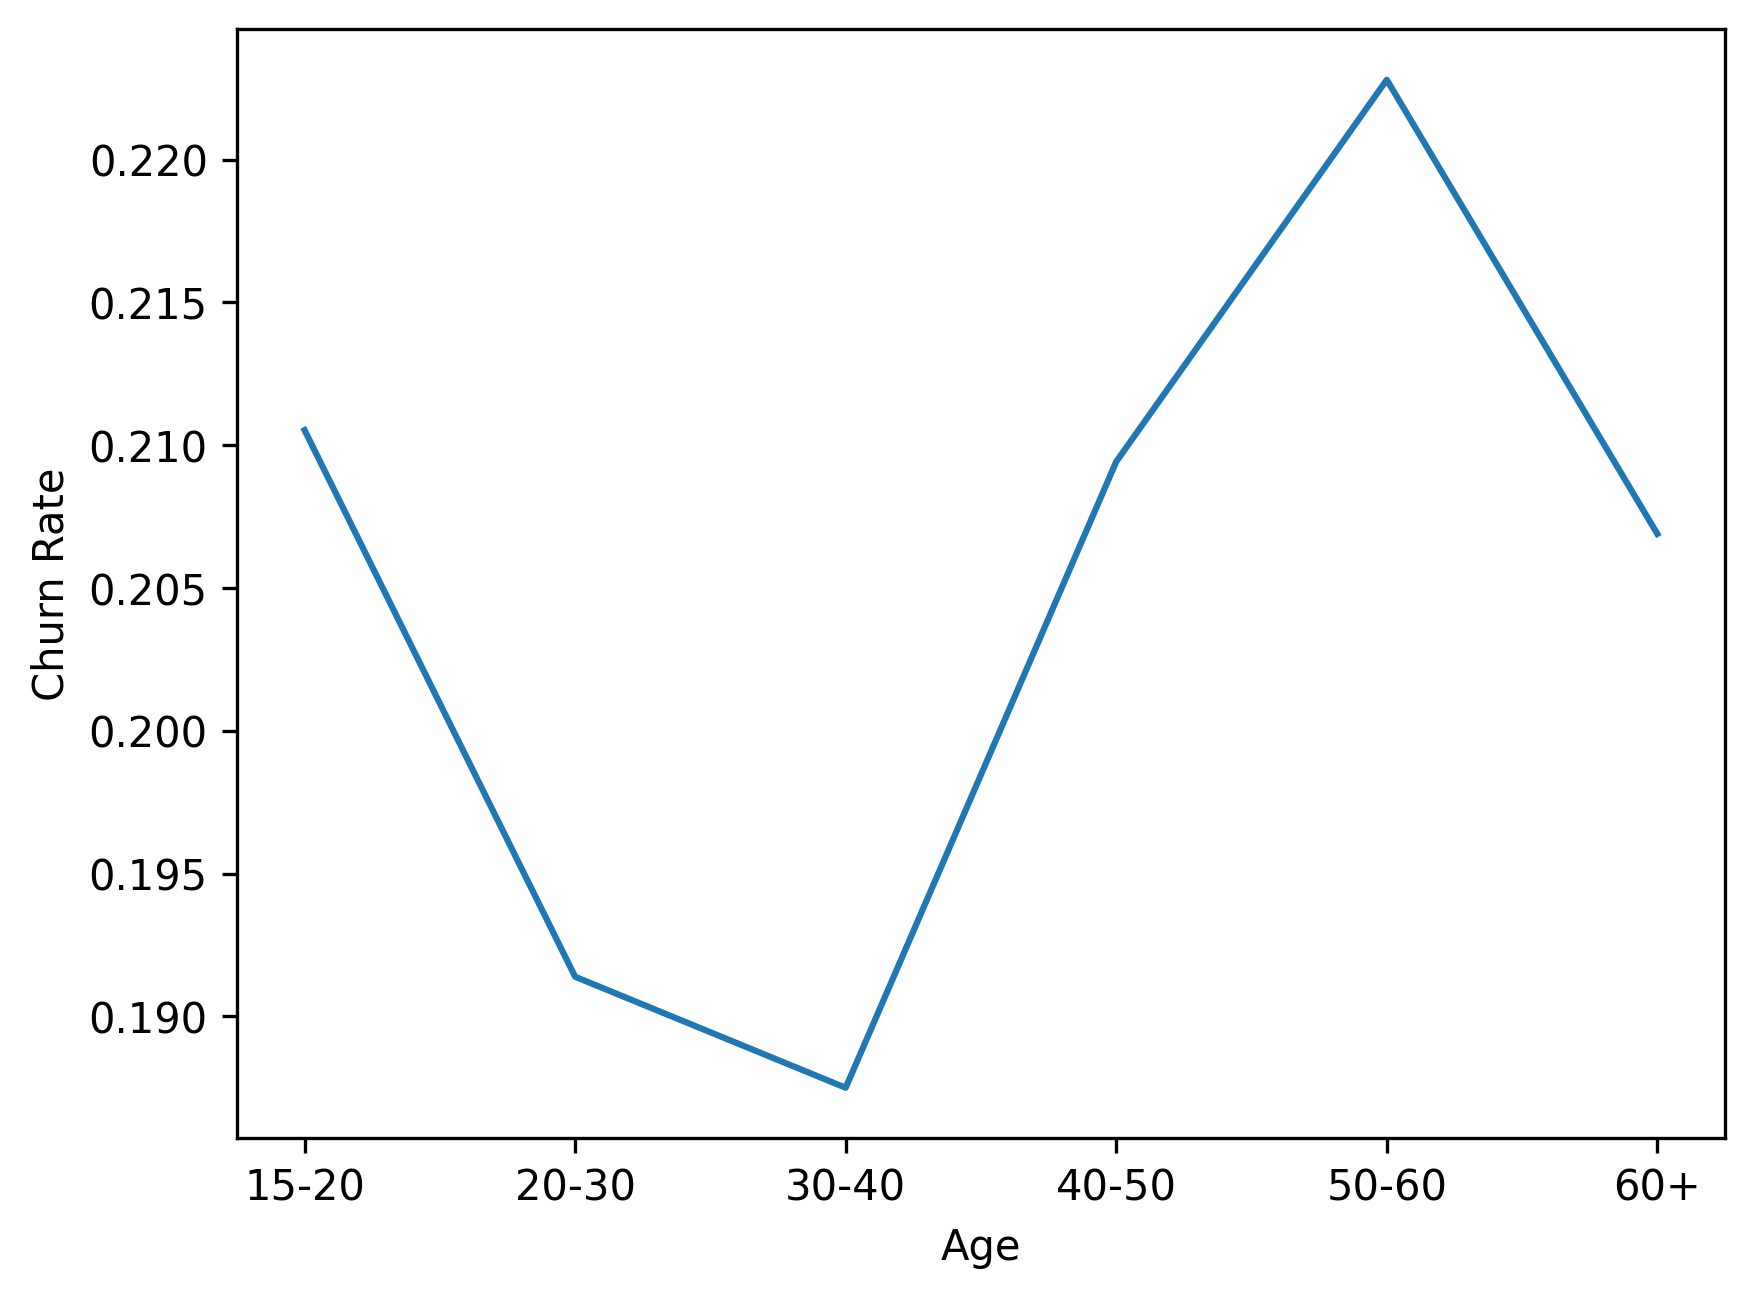
\includegraphics[width=0.6\textwidth]{Plots/agerange_churn_rate.png} 
    \caption{Churn Rate by Age Range with binning}
    \label{fig:agerange_churn}
\end{figure}

As shown in Fig~\ref{fig:agerange_churn}, it indicates groups in 20-30 and 30-40 have a relatively low churn rate compared to other groups. This trend may be attributed to their stable income levels, which contribute to higher customer retention.

To emphasise this trend among different groups for later analysis, the Z-score is caculated for each group with:

\begin{equation}
\mathcal{Z} =  \frac{X - \mu}{\sigma}
\label{eq1}
\end{equation}

where X is the average churn rate in each group, $\mu$ and $\sigma$ are the mean value and standard variance of churn rate.

For effective transformation from categorical to numerical data, one-hot encoding~\cite{poslavskaya2023encodingcategoricaldatahotter} is applied to variables such as Gender, MaritalStatus, and IncomeLevel, which convert each category into a binary vector representation without introducing unintended ordinal relationships.




\subsection{Customer Interaction}

In the Interaction sheet, three different interaction categories are recorded: feedback, inquiry, and complaint. Each interaction has a corresponding ResolutionStatus, which is either solved or unsolved.

\begin{figure}[h]
    \centering
    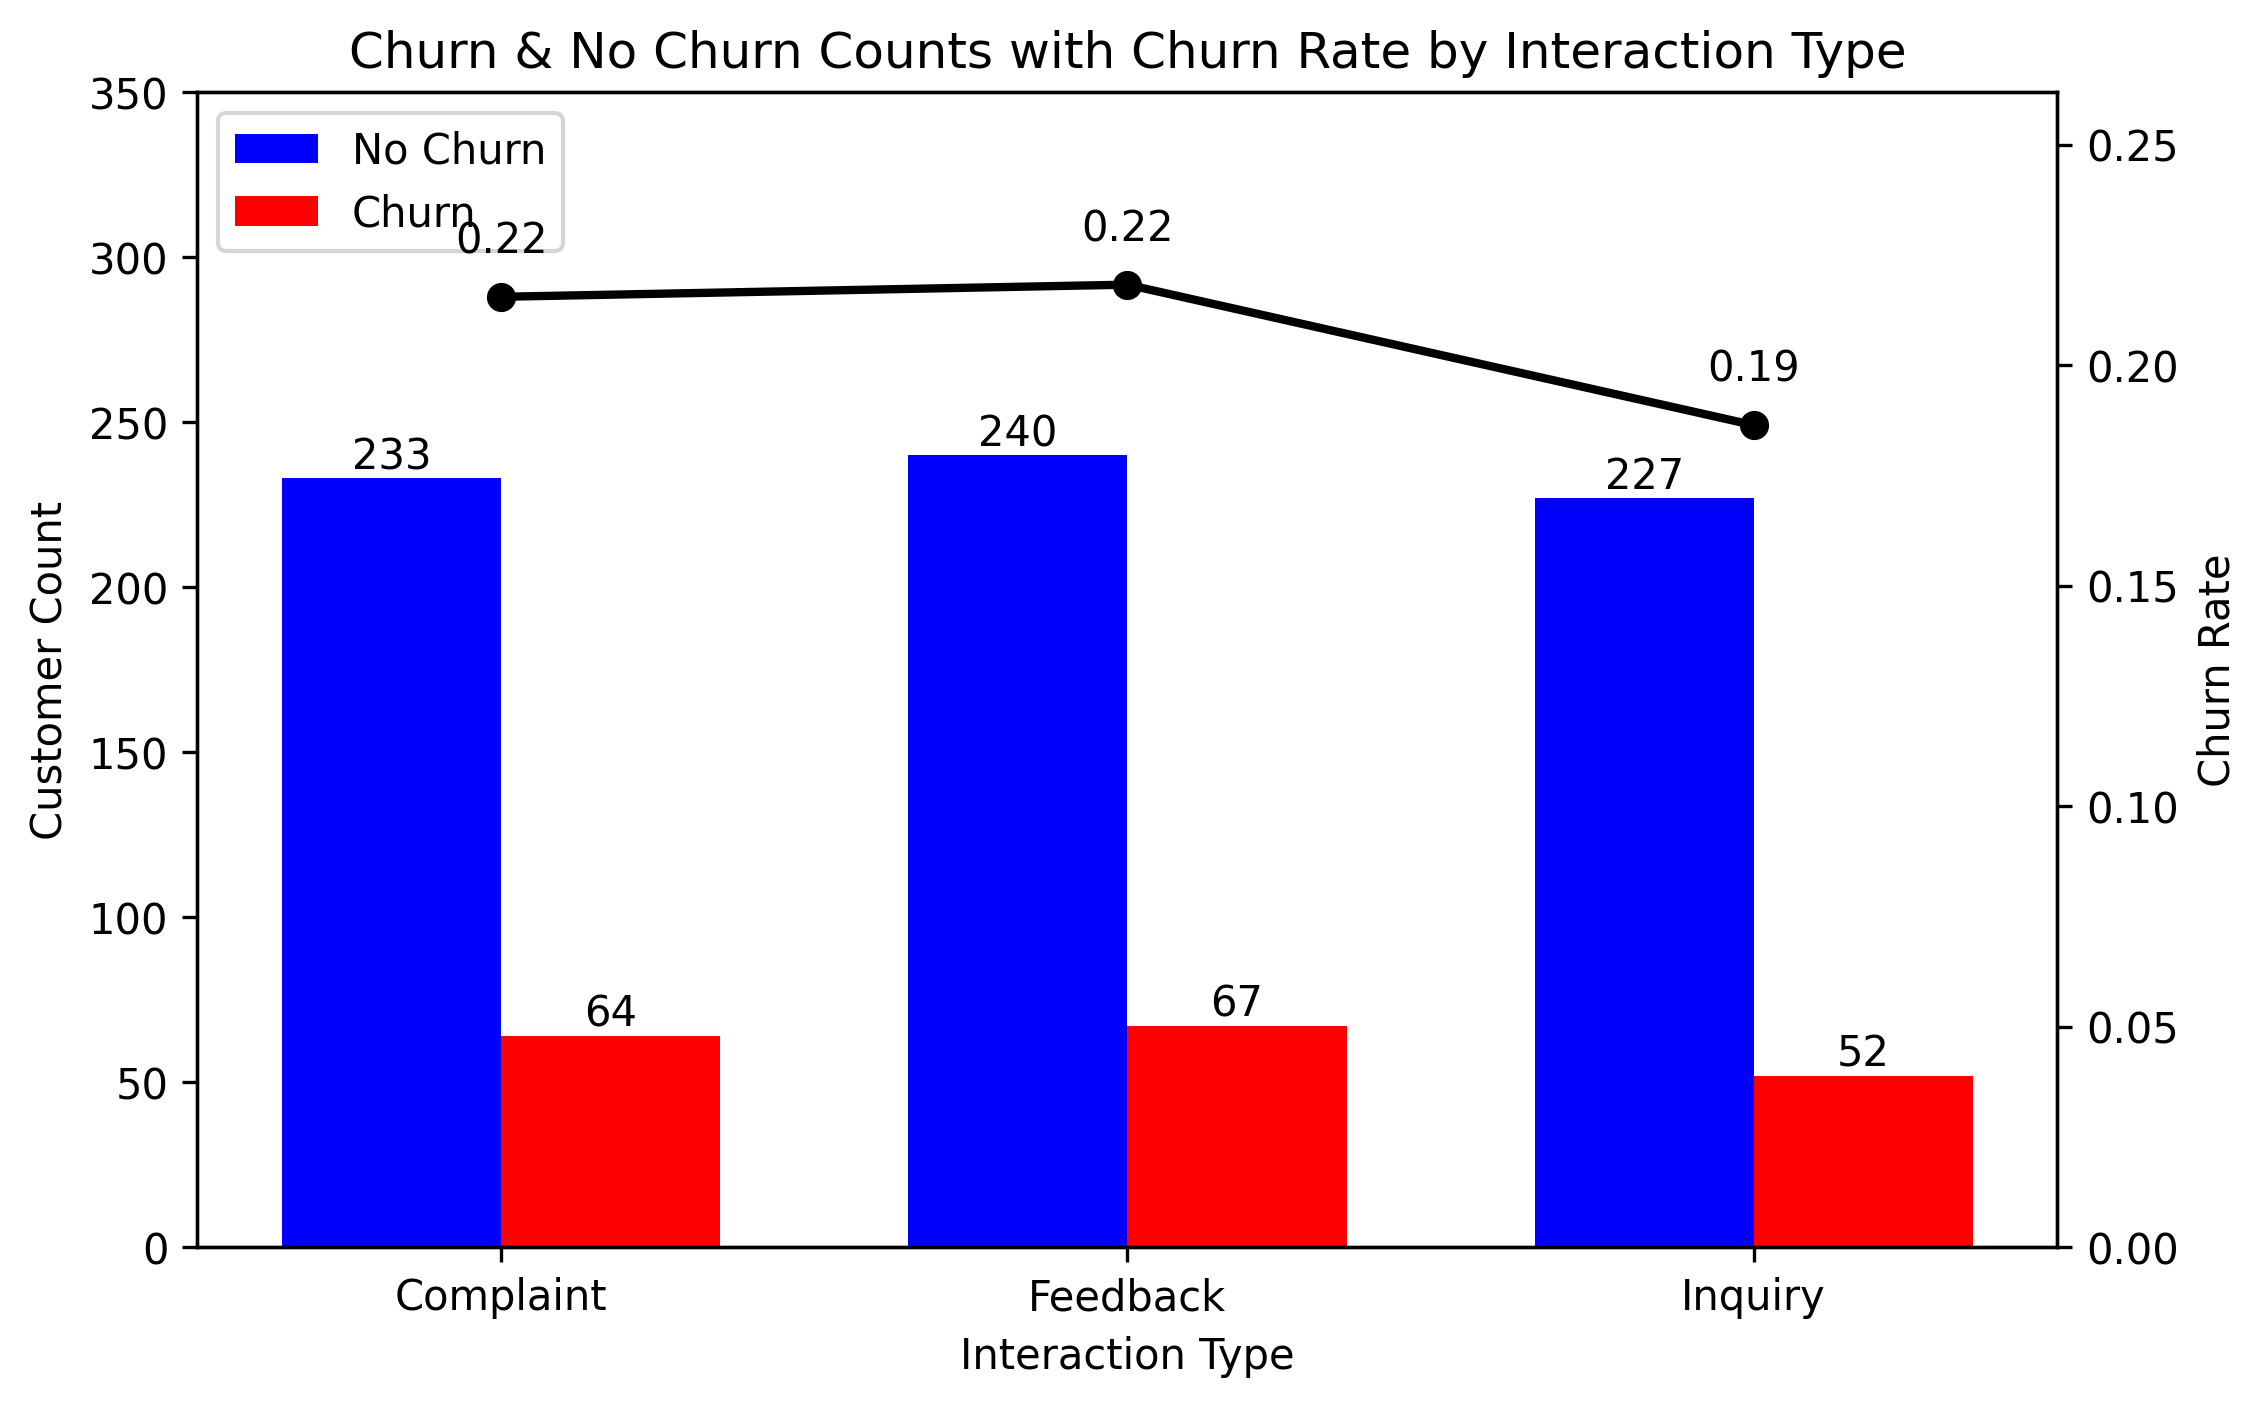
\includegraphics[width=0.49\textwidth]{Plots/churn_rate_interactiontype.png} 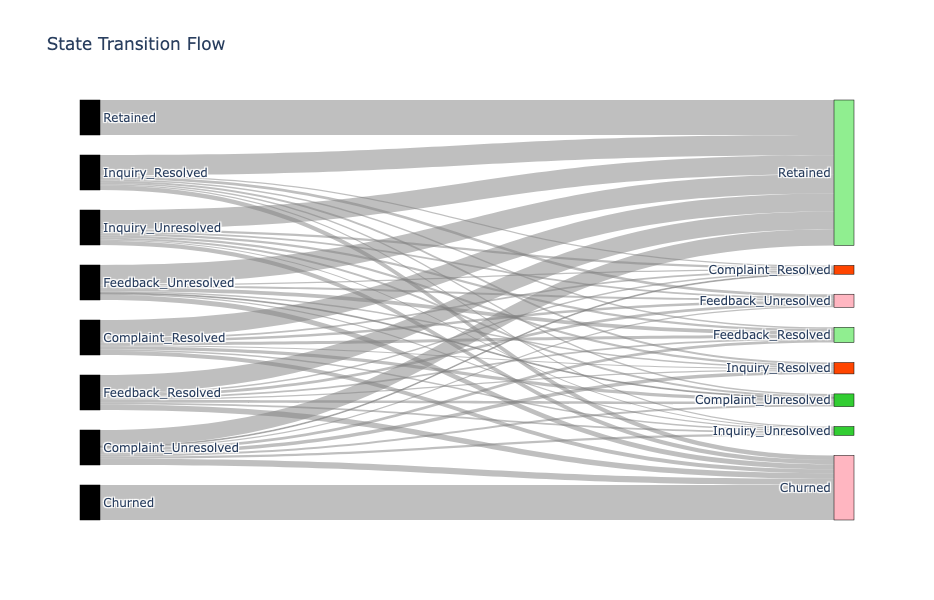
\includegraphics[width=0.49\textwidth]{Plots/flow_interaction.png}
    \caption{Interaction Type Counts with Churn Rates (left) and state transition Flow (right)}
    \label{fig:interactiontype_churn}
\end{figure}

Although the inquiry shows a lower churn rate as shown in Fig~\ref{fig:interactiontype_churn}, it may not be a real situation without considering the ResolutionStatus. For example, successfully resolved inquiries are likely to increase customer retention. To more accurately model this process, a Markov Chain is applied. To avoid the complexity of higher-order chains while preserving key interaction patterns, a combined feature of InteractionType and ResolutionStatus is introduced.

The customer journey begins with a specific type of interaction and progresses through various states based on their interaction types and resolution outcomes. Finally, the customer transitions into one of two absorbing states, either churned or retained, where they remain indefinitely, as shown in Fig~\ref{fig:interactiontype_chain}.

\begin{figure}[h]
    \centering
    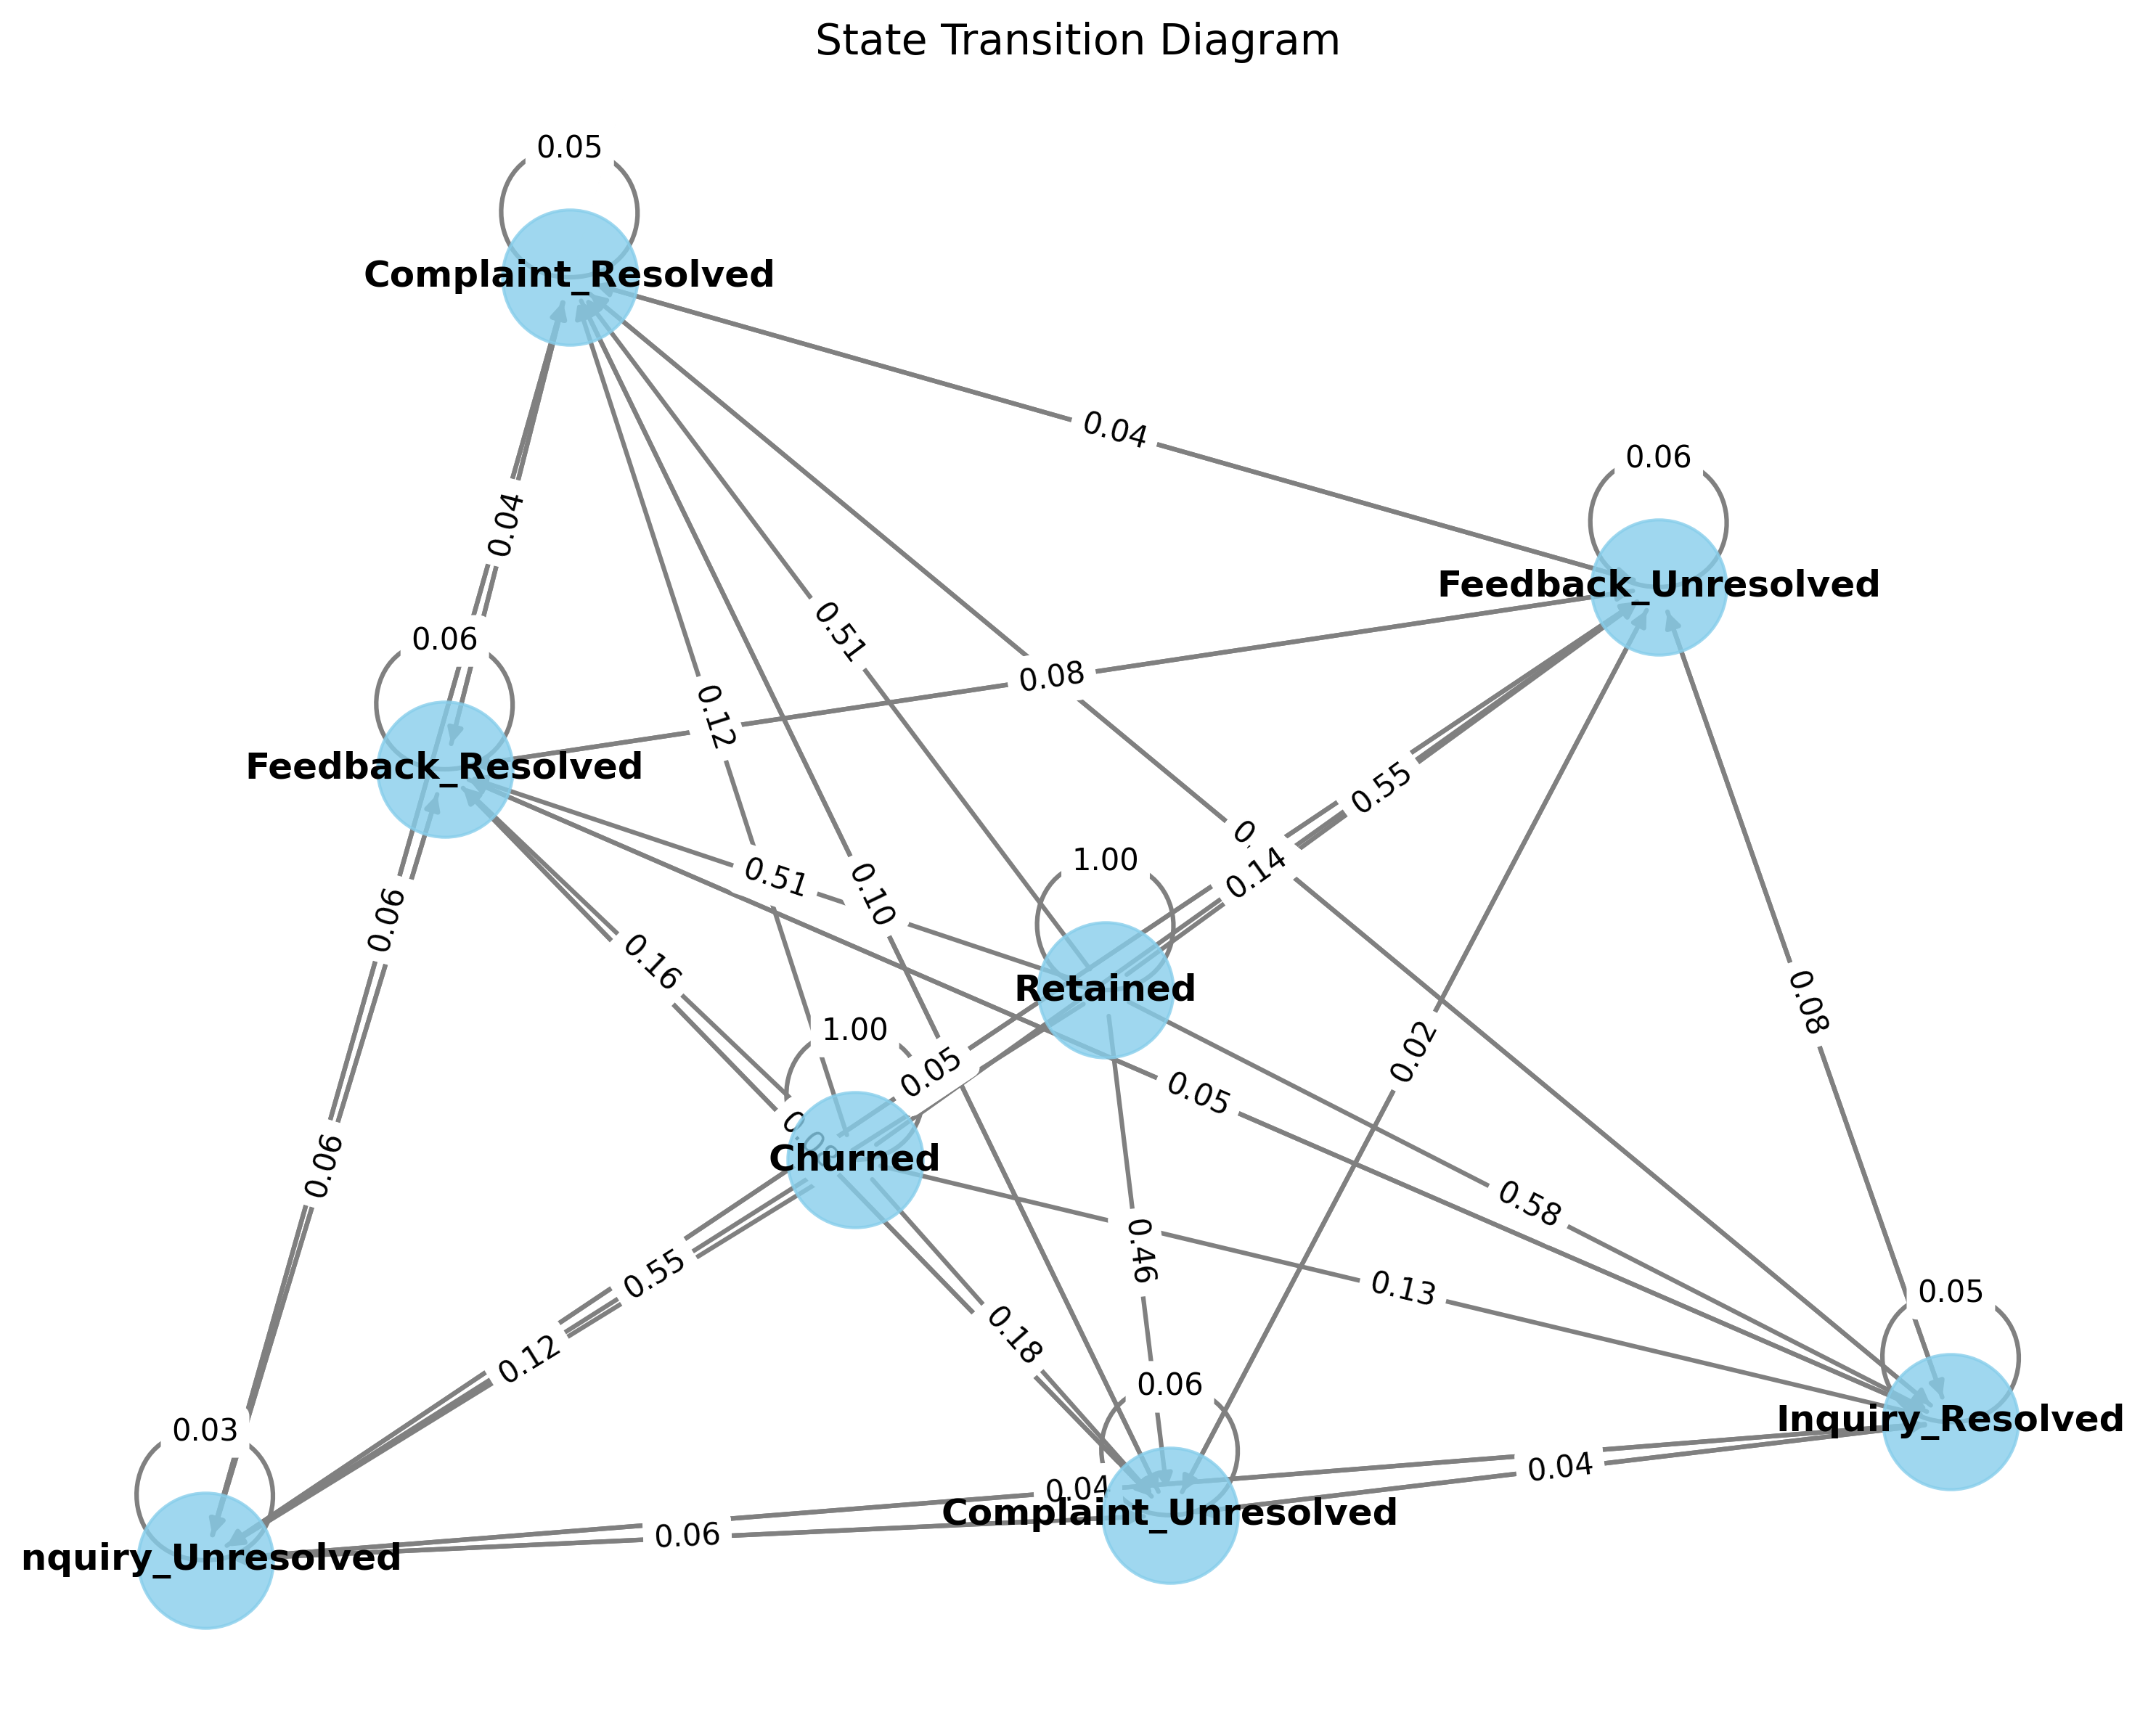
\includegraphics[width=0.8\textwidth]{Plots/chain_interactiontype.png}
    
    \caption{State Trasition Chain with combined features}
    \label{fig:interactiontype_chain}
\end{figure}

\begin{figure}[h]
    \centering
    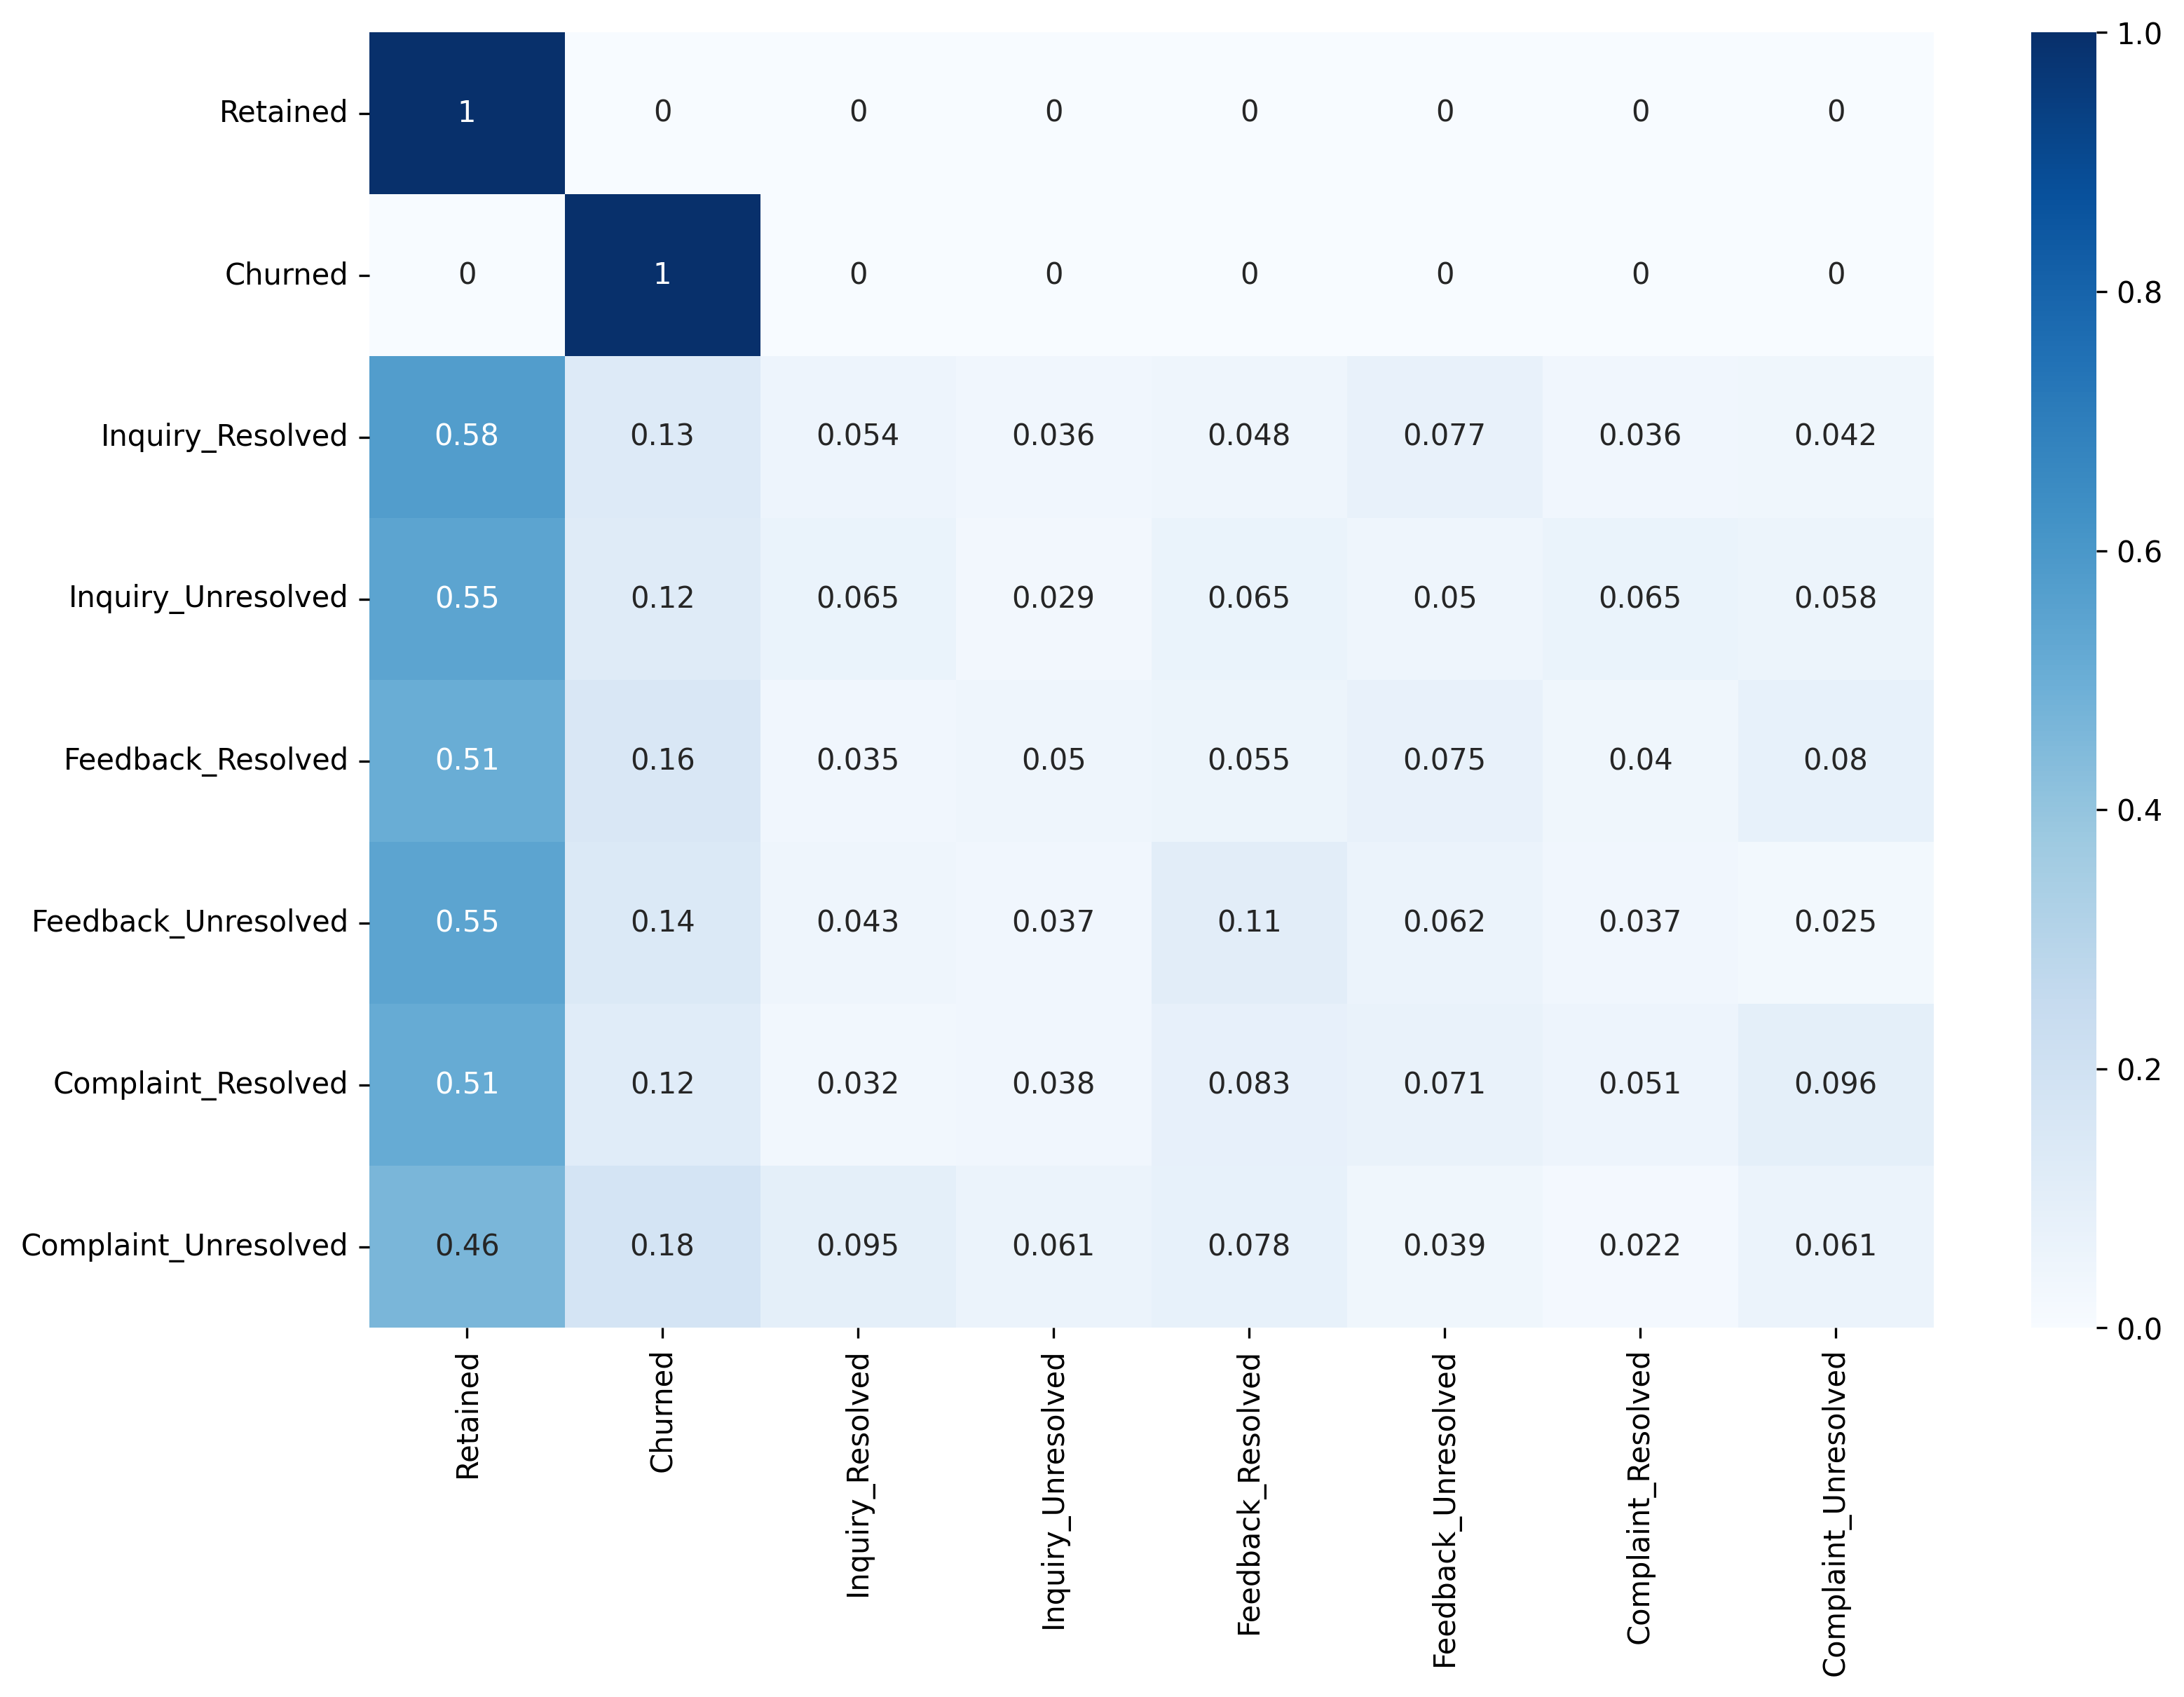
\includegraphics[width=0.8\textwidth]{Plots/transition_matrix.png}
    
    \caption{Trasition Matrix with combined features}
    \label{fig:transition_matrix}
\end{figure}

The transition matrix can also be calculated as shown in Fig~\ref{fig:transition_matrix}, and we can calculate absorption probabilities for the recurrent class with formula ~\ref{eq2}:
\begin{equation}
\begin{aligned}
F & =(I-T)^{-1} S \\
& =U S
\label{eq2}
\end{aligned}
\end{equation}

\begin{table}[h]
    \centering
    \begin{tabular}{c|c|c}
        \hline
        \textbf{State} & \textbf{Retention Probability} & \textbf{Churn Probability} \\
        \hline
        Inquiry Resolved & 0.8070 & 0.1930 \\
        Inquiry Unresolved & 0.8068 & 0.1932 \\
        Feedback Resolved & 0.7708 & 0.2292 \\
        Feedback Unresolved & 0.7906 & 0.2094 \\
        Complaint Resolved & 0.8025 & 0.1975 \\
        Complaint Unresolved & 0.7448 & 0.2552 \\
        \hline \\
    \end{tabular}
    \caption{Absorption Probability Matrix (F)}
    \label{tab:absorb_prob_matrix}
\end{table}

Among all states, Complaint Unresolved has the highest churn probability (25.52\%), suggesting that unresolved complaints are a significant risk factor for customer attrition. Conversely, Inquiry Resolved and Inquiry Unresolved show relatively lower churn probabilities (19.30\% and 19.32\%, respectively). To account for this, a new feature is introduced that assigns a churn probability based on each customer's final interaction type as shown in Tab~\ref{tab:absorb_prob_matrix}.

Furthermore, churn status is influenced not only by the most recent interaction but also by prior interactions. To capture this relationship, additional features are engineered, such as the frequency of each interaction type, resolution status, and duration between interactions.

\subsection{Transaction History}

The Transaction Sheet provides insights into hidden consumption behaviours. To analyse customer activity levels, key metrics such as minimum, maximum, total spending, average transaction value, and transaction count are calculated. These metrics help quantify purchase frequency, spending patterns, and overall engagement.

Moreover, analysing customer spending behaviour across different product categories can help uncover valuable insights for churn prediction. A natural approach is to analyse consumer spending patterns across different product categories within a short time window while considering their churn status. 

As shown in Fig~\ref{fig:violin_total}, churned customers have a smaller total spent, and Fig.~\ref{fig:KDE} illustrates the differences in short-time purchasing behaviour between retained and churned customers, showing that churned customers tend to spend less on electronics and clothing. To better capture these patterns, proper binning is applied to categorise customers based on their spending range. 


\begin{figure}[h]
    \centering
    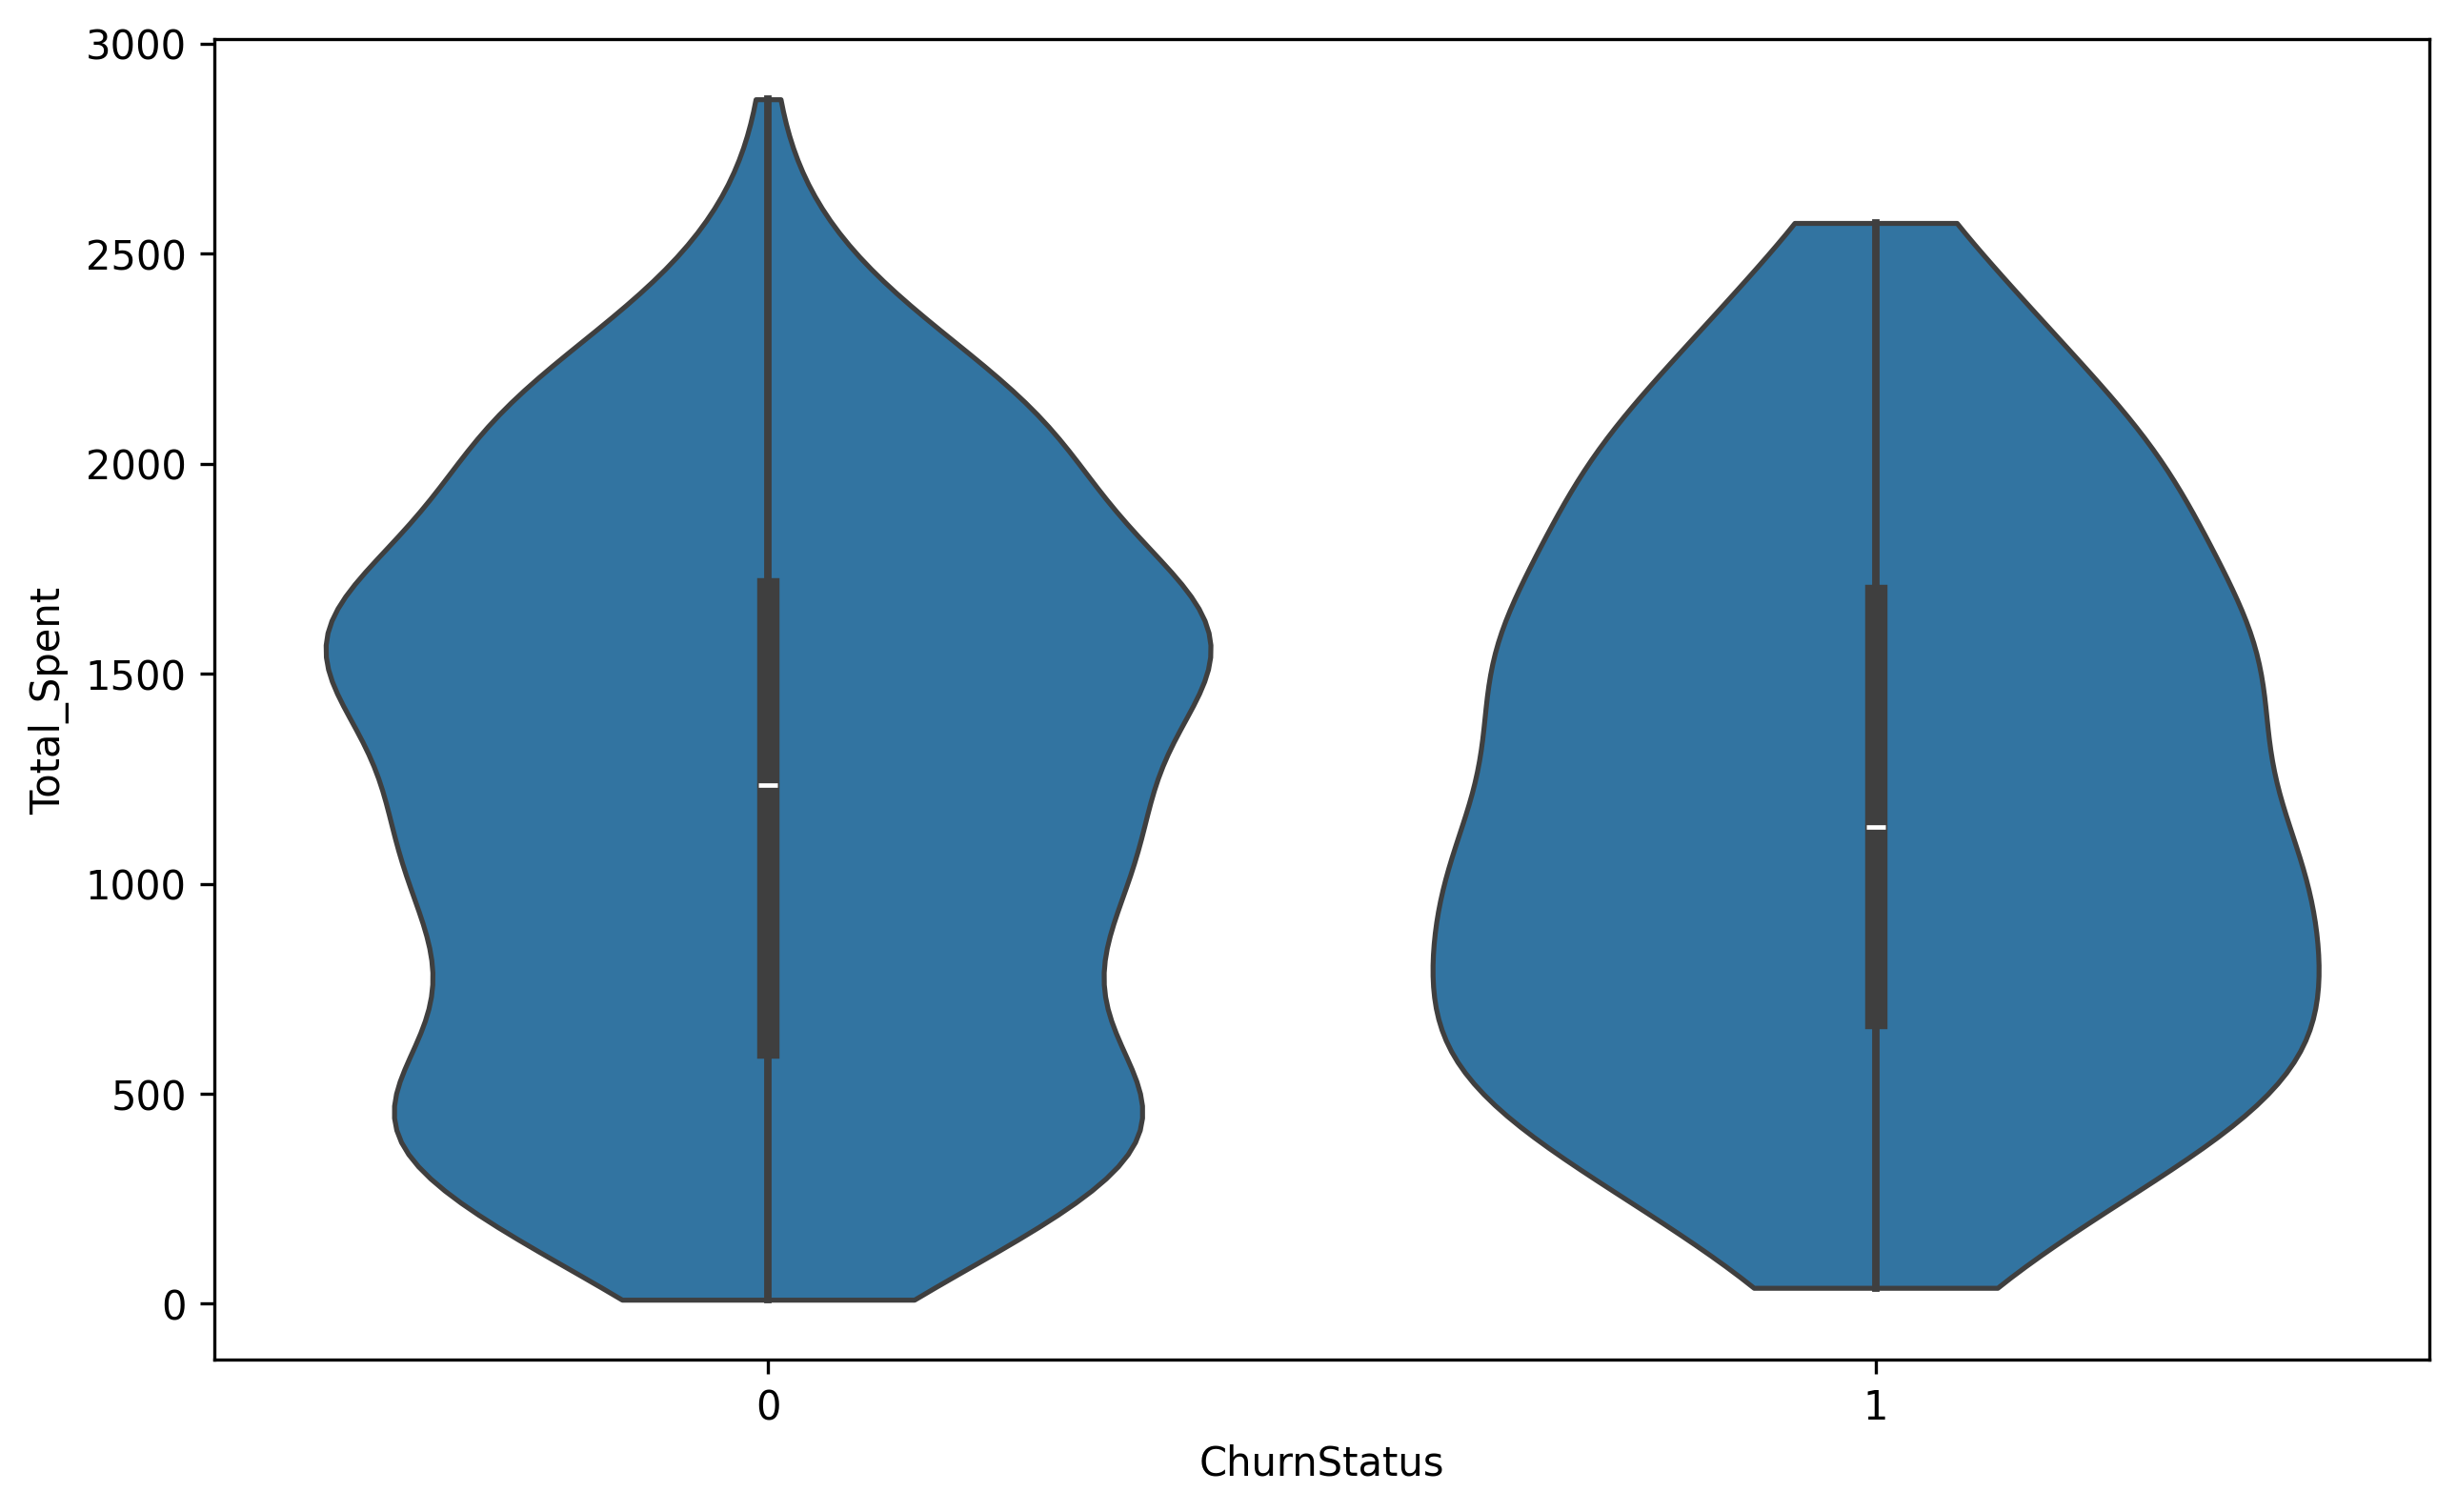
\includegraphics[width=0.5\textwidth]{Plots/violin_total_spent.png}
    \caption{Distribution of total transaction for churned and retained customer}
    \label{fig:violin_total}
\end{figure}

\begin{figure}[h]
    \centering
    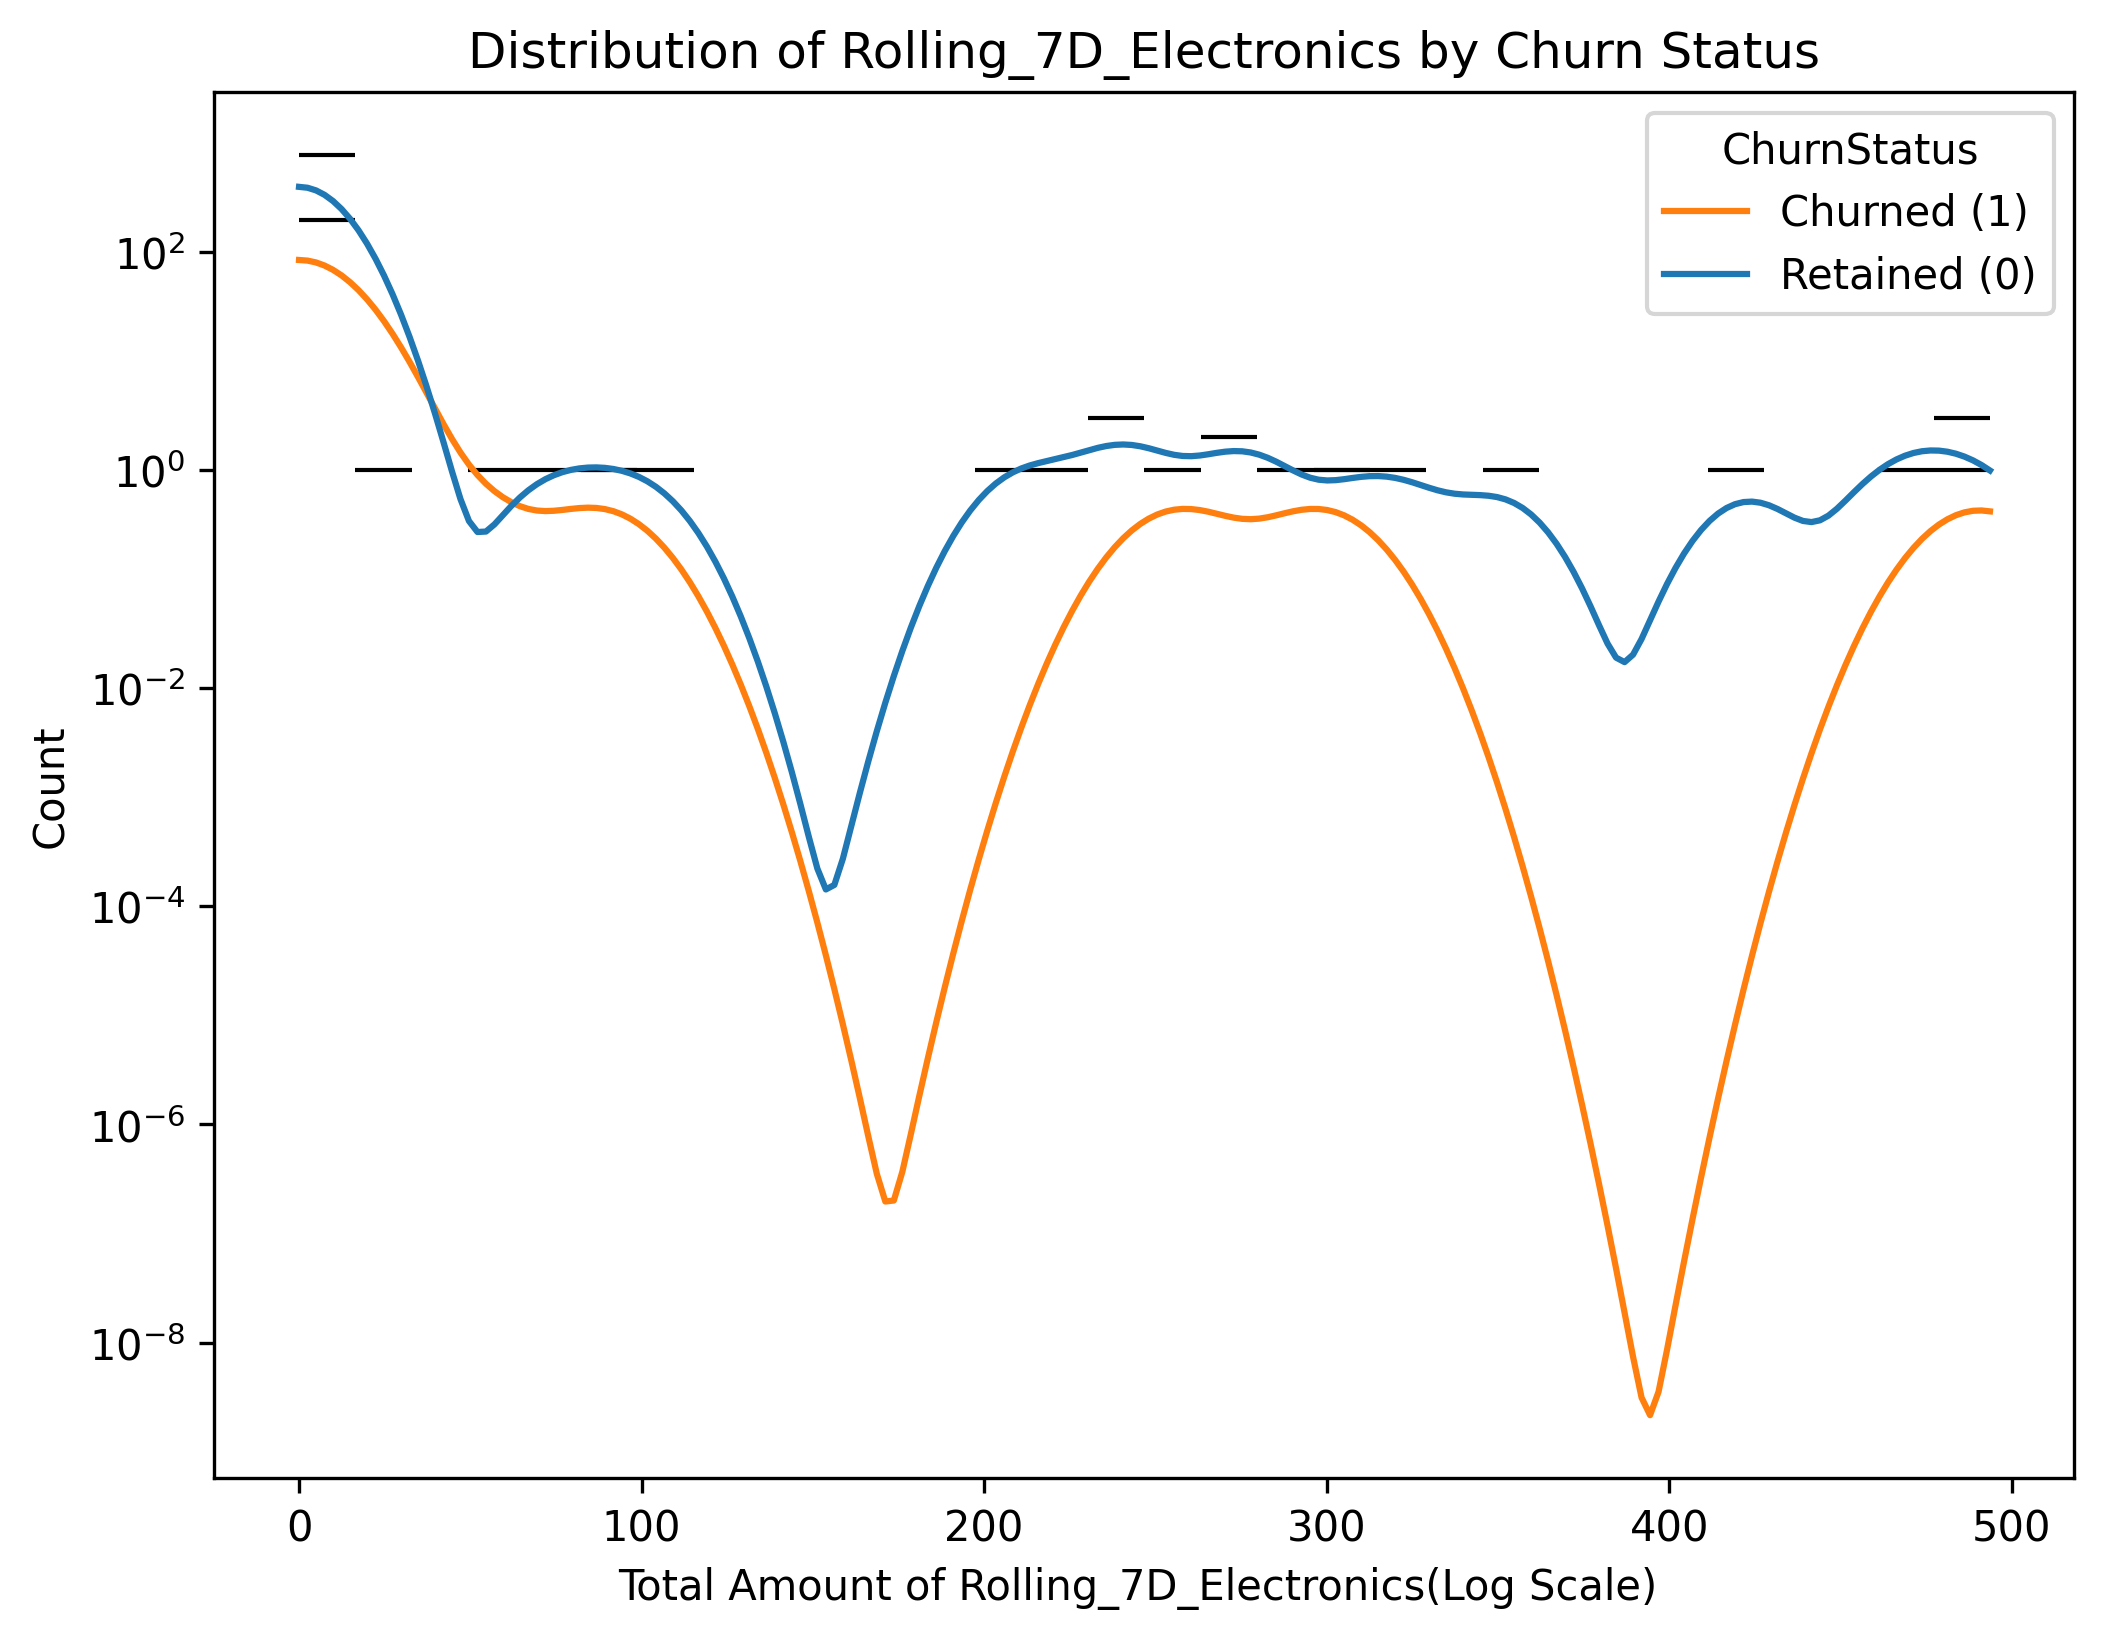
\includegraphics[width=0.49\textwidth]{Plots/KDE_RollingElectronics.png}
    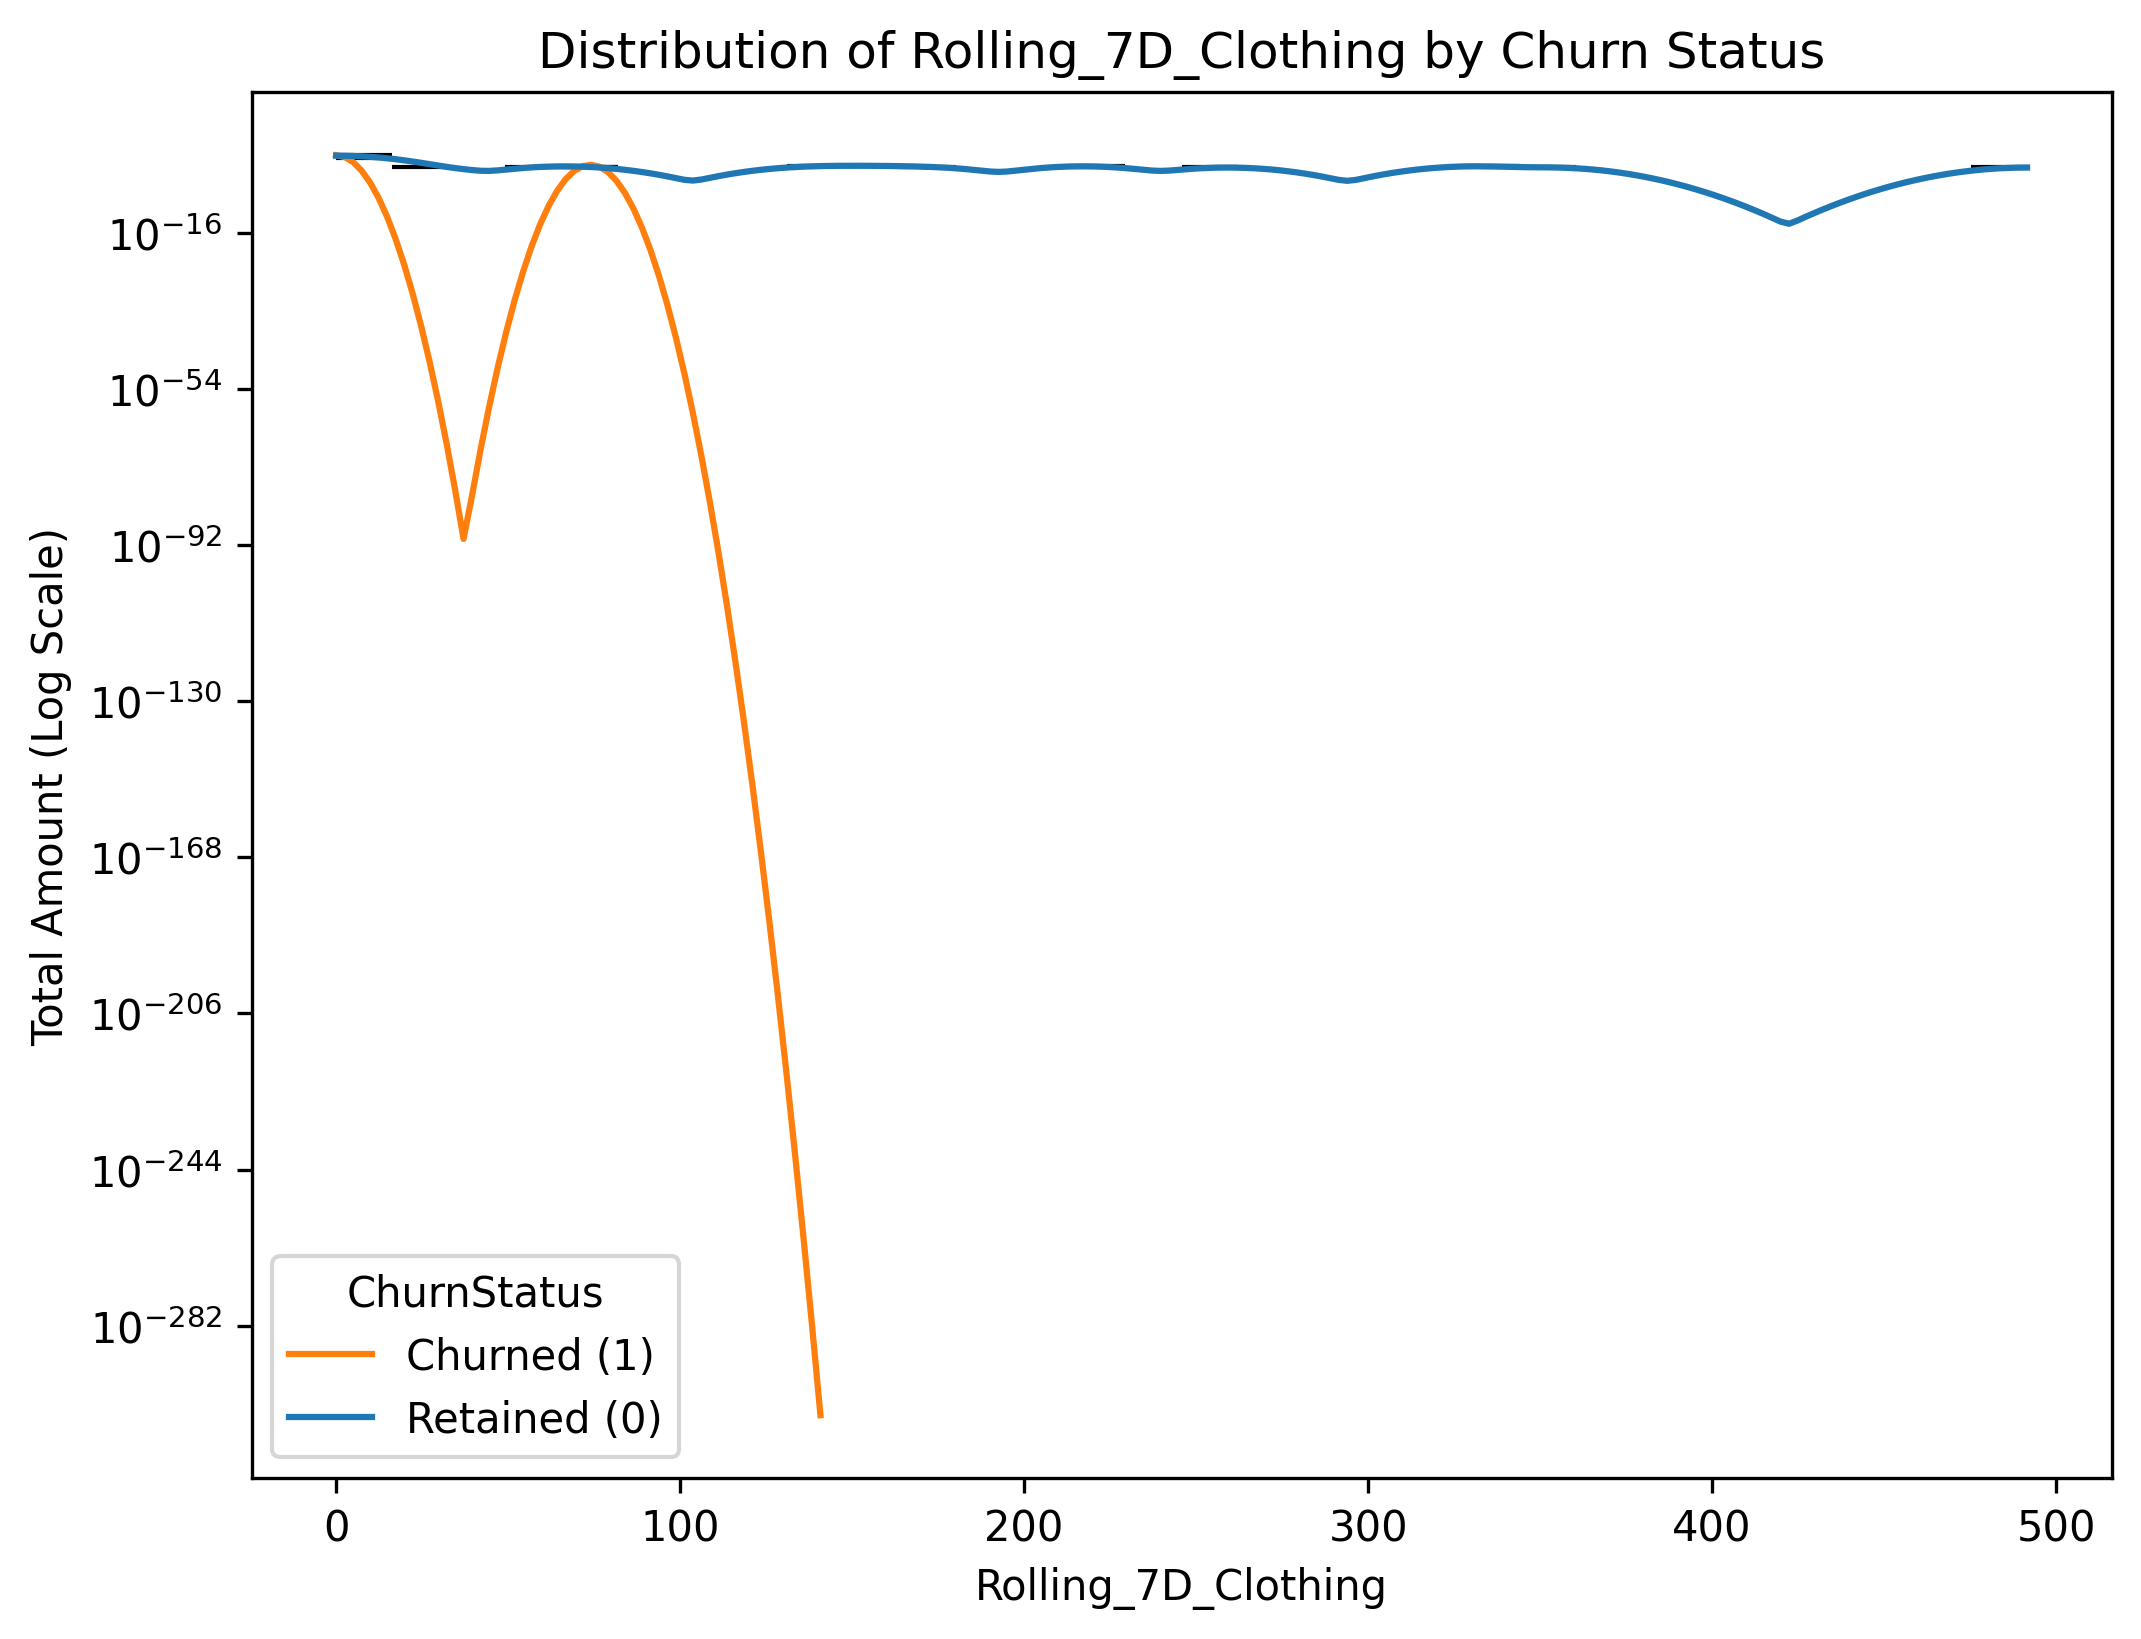
\includegraphics[width=0.49\textwidth]{Plots/KDE_RollingClothing.png}
    \caption{KDE plots for short-term spending patterns in electronics (left) and clothing (right). }
    \label{fig:KDE}
\end{figure}

The bining settings for five different products are shown in Tab~\ref{tab:bining_summary}.

\begin{table}[h]
    \centering
    \begin{tabular}{c|c}
        \hline
        \textbf{Product Category} & \textbf{bining settings} \\
        \hline
        Furniture &  [0, 100, 210, $\infty$] \\
        \hline
        Clothing &  [0, 10, 40, 150, $\infty$] \\
        \hline
        Electronics &  [0, 160, 200, 310, 360, 420, 440, $\infty$] \\
        \hline
        Books &  [0, 80, 220, $\infty$] \\
        \hline
        Groceries & [0, 80, 200, 280, 320, 380, 410, $\infty$]  \\
        \hline \\
    \end{tabular}
    \caption{Summary of bining settings for each products based on KDE distributions}
    \label{tab:bining_summary}
\end{table}


\subsection{Login Activity}
The Login Activity sheet contains three key features: LastLoginDate, LoginFrequency, and ServiceUsage. To transform LastLoginDate into numerical data, we can calculate the difference between each entry and the maximum LastLoginDate in the dataset. Once transformed, we can apply a t-test to determine whether there are significant differences in feature mean values between users with different ChurnStatus.

For category variable ServiceUsage, $\chi^2$ statistics can be calculated to indicate whether there is a relationship with ChurnStatus.

\begin{figure}[h]
    \centering
    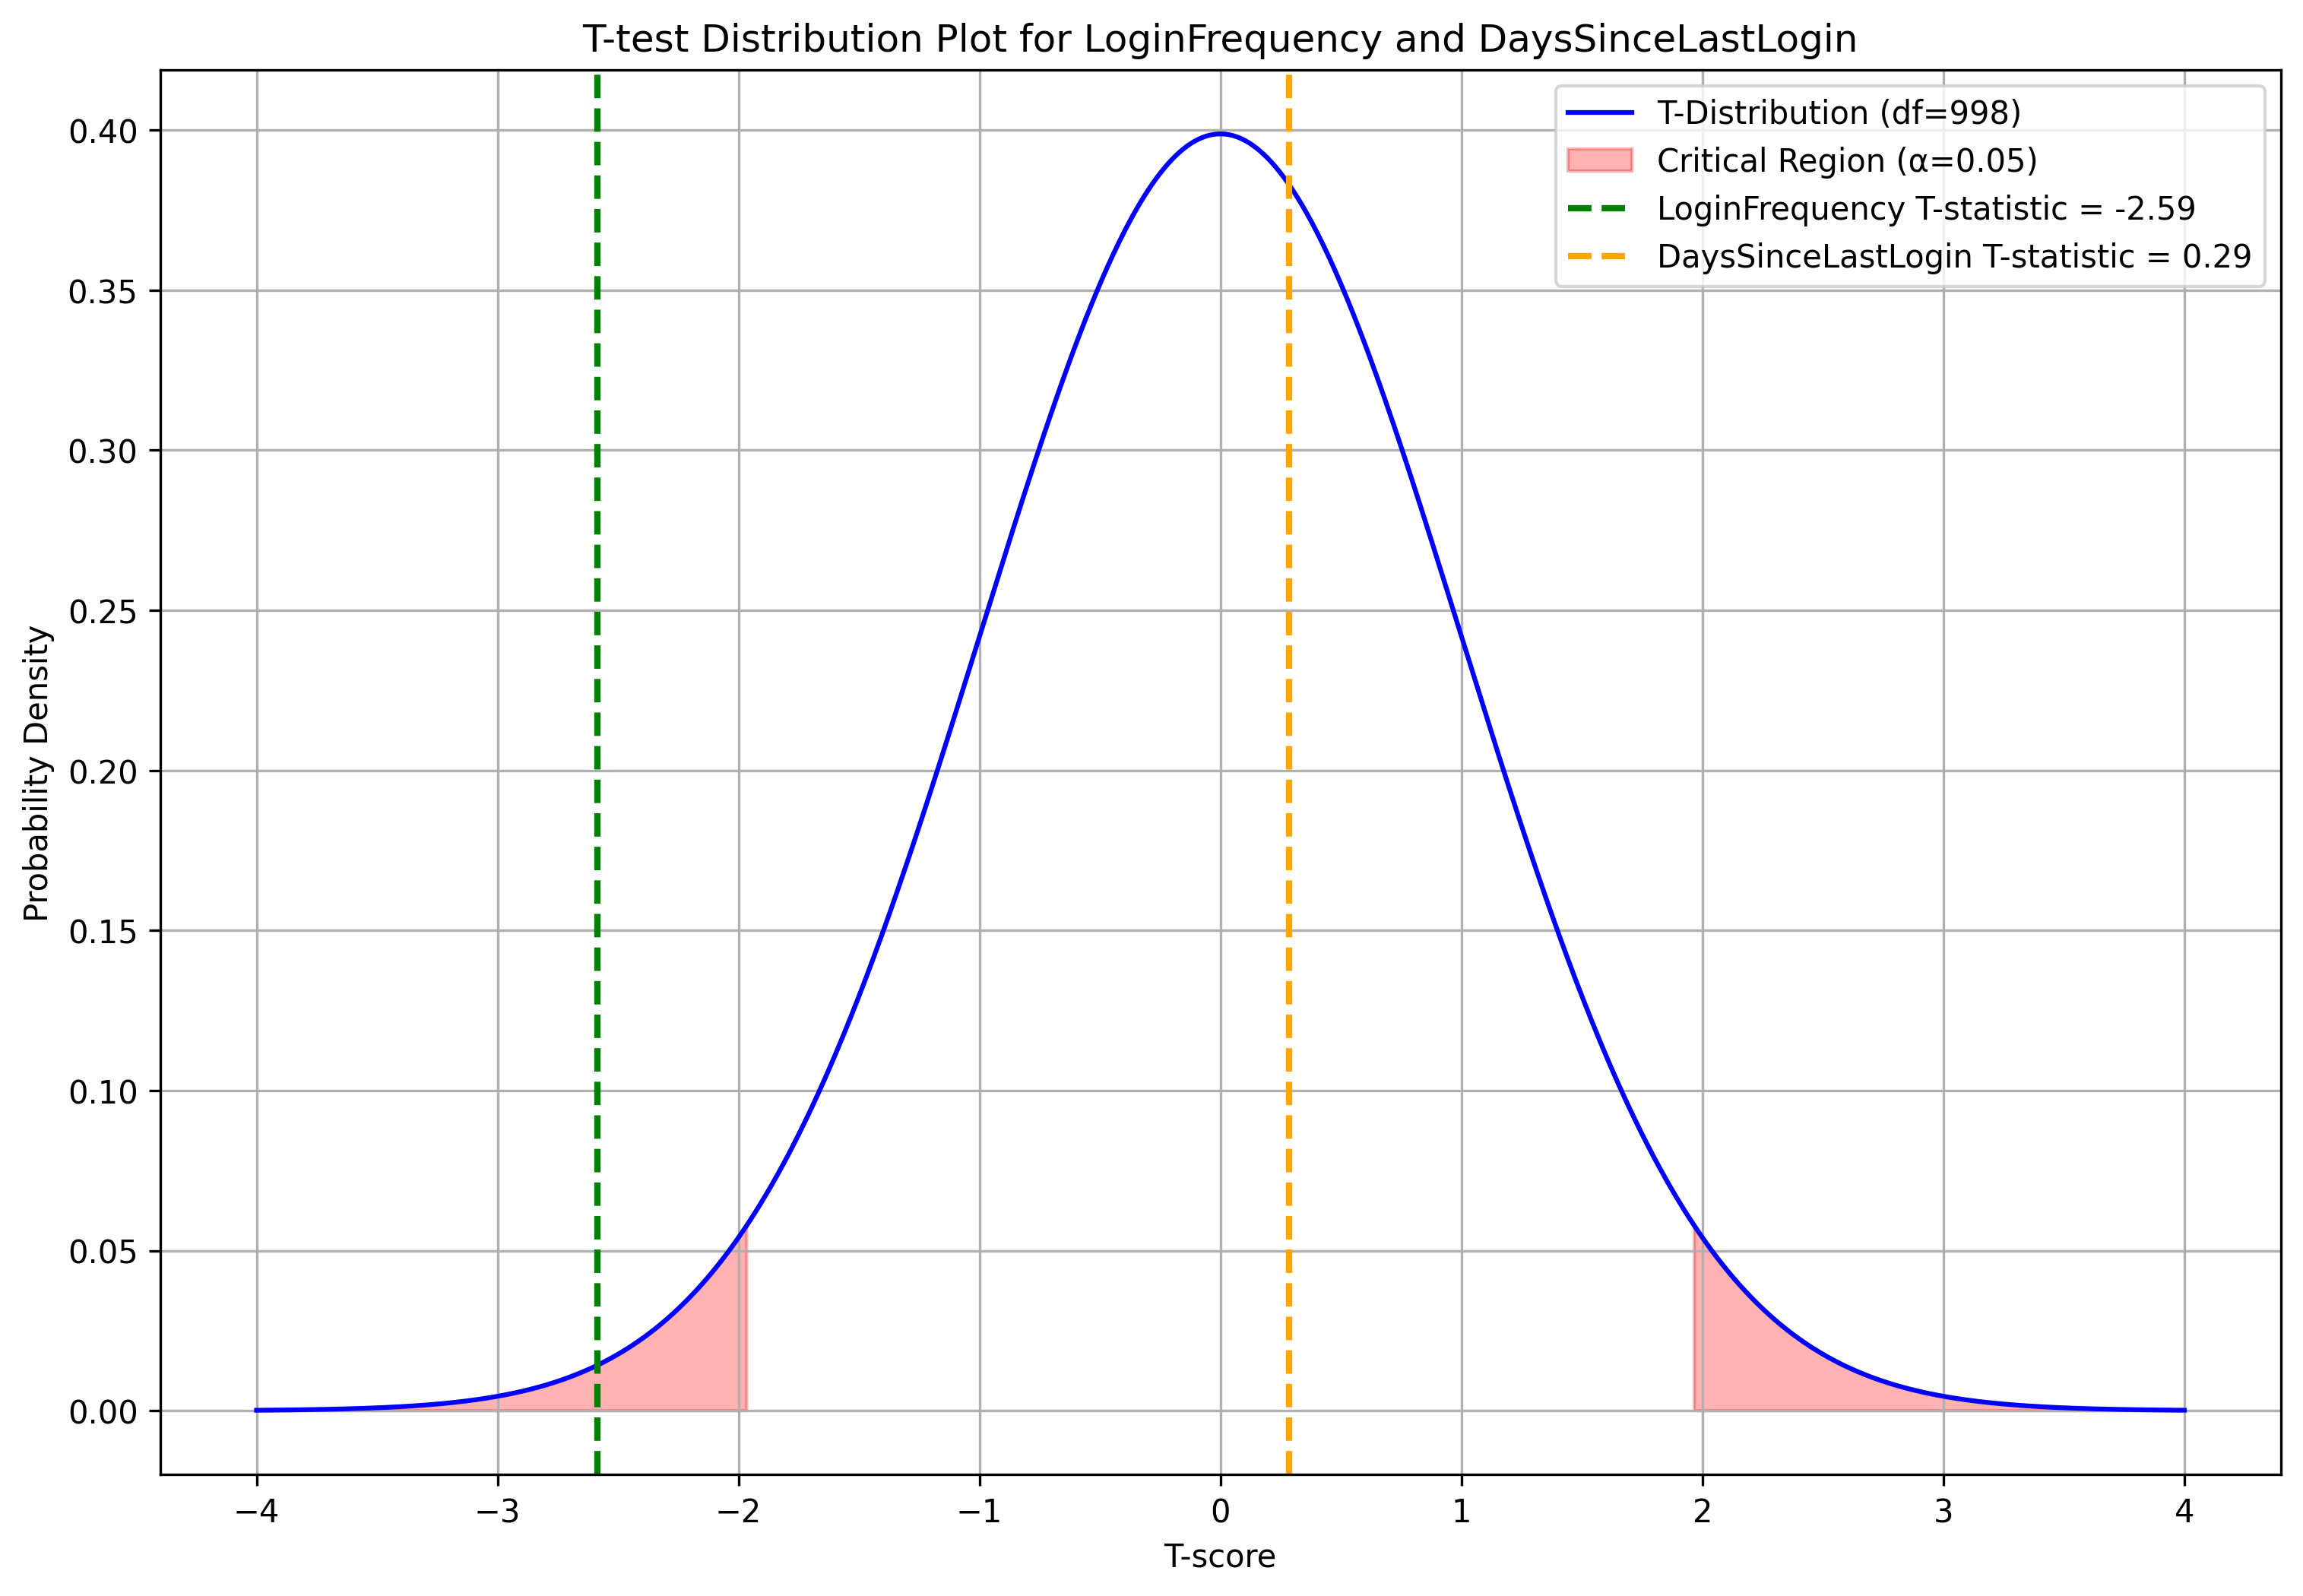
\includegraphics[width=0.49\textwidth]{Plots/T_test_Distribution.png}
    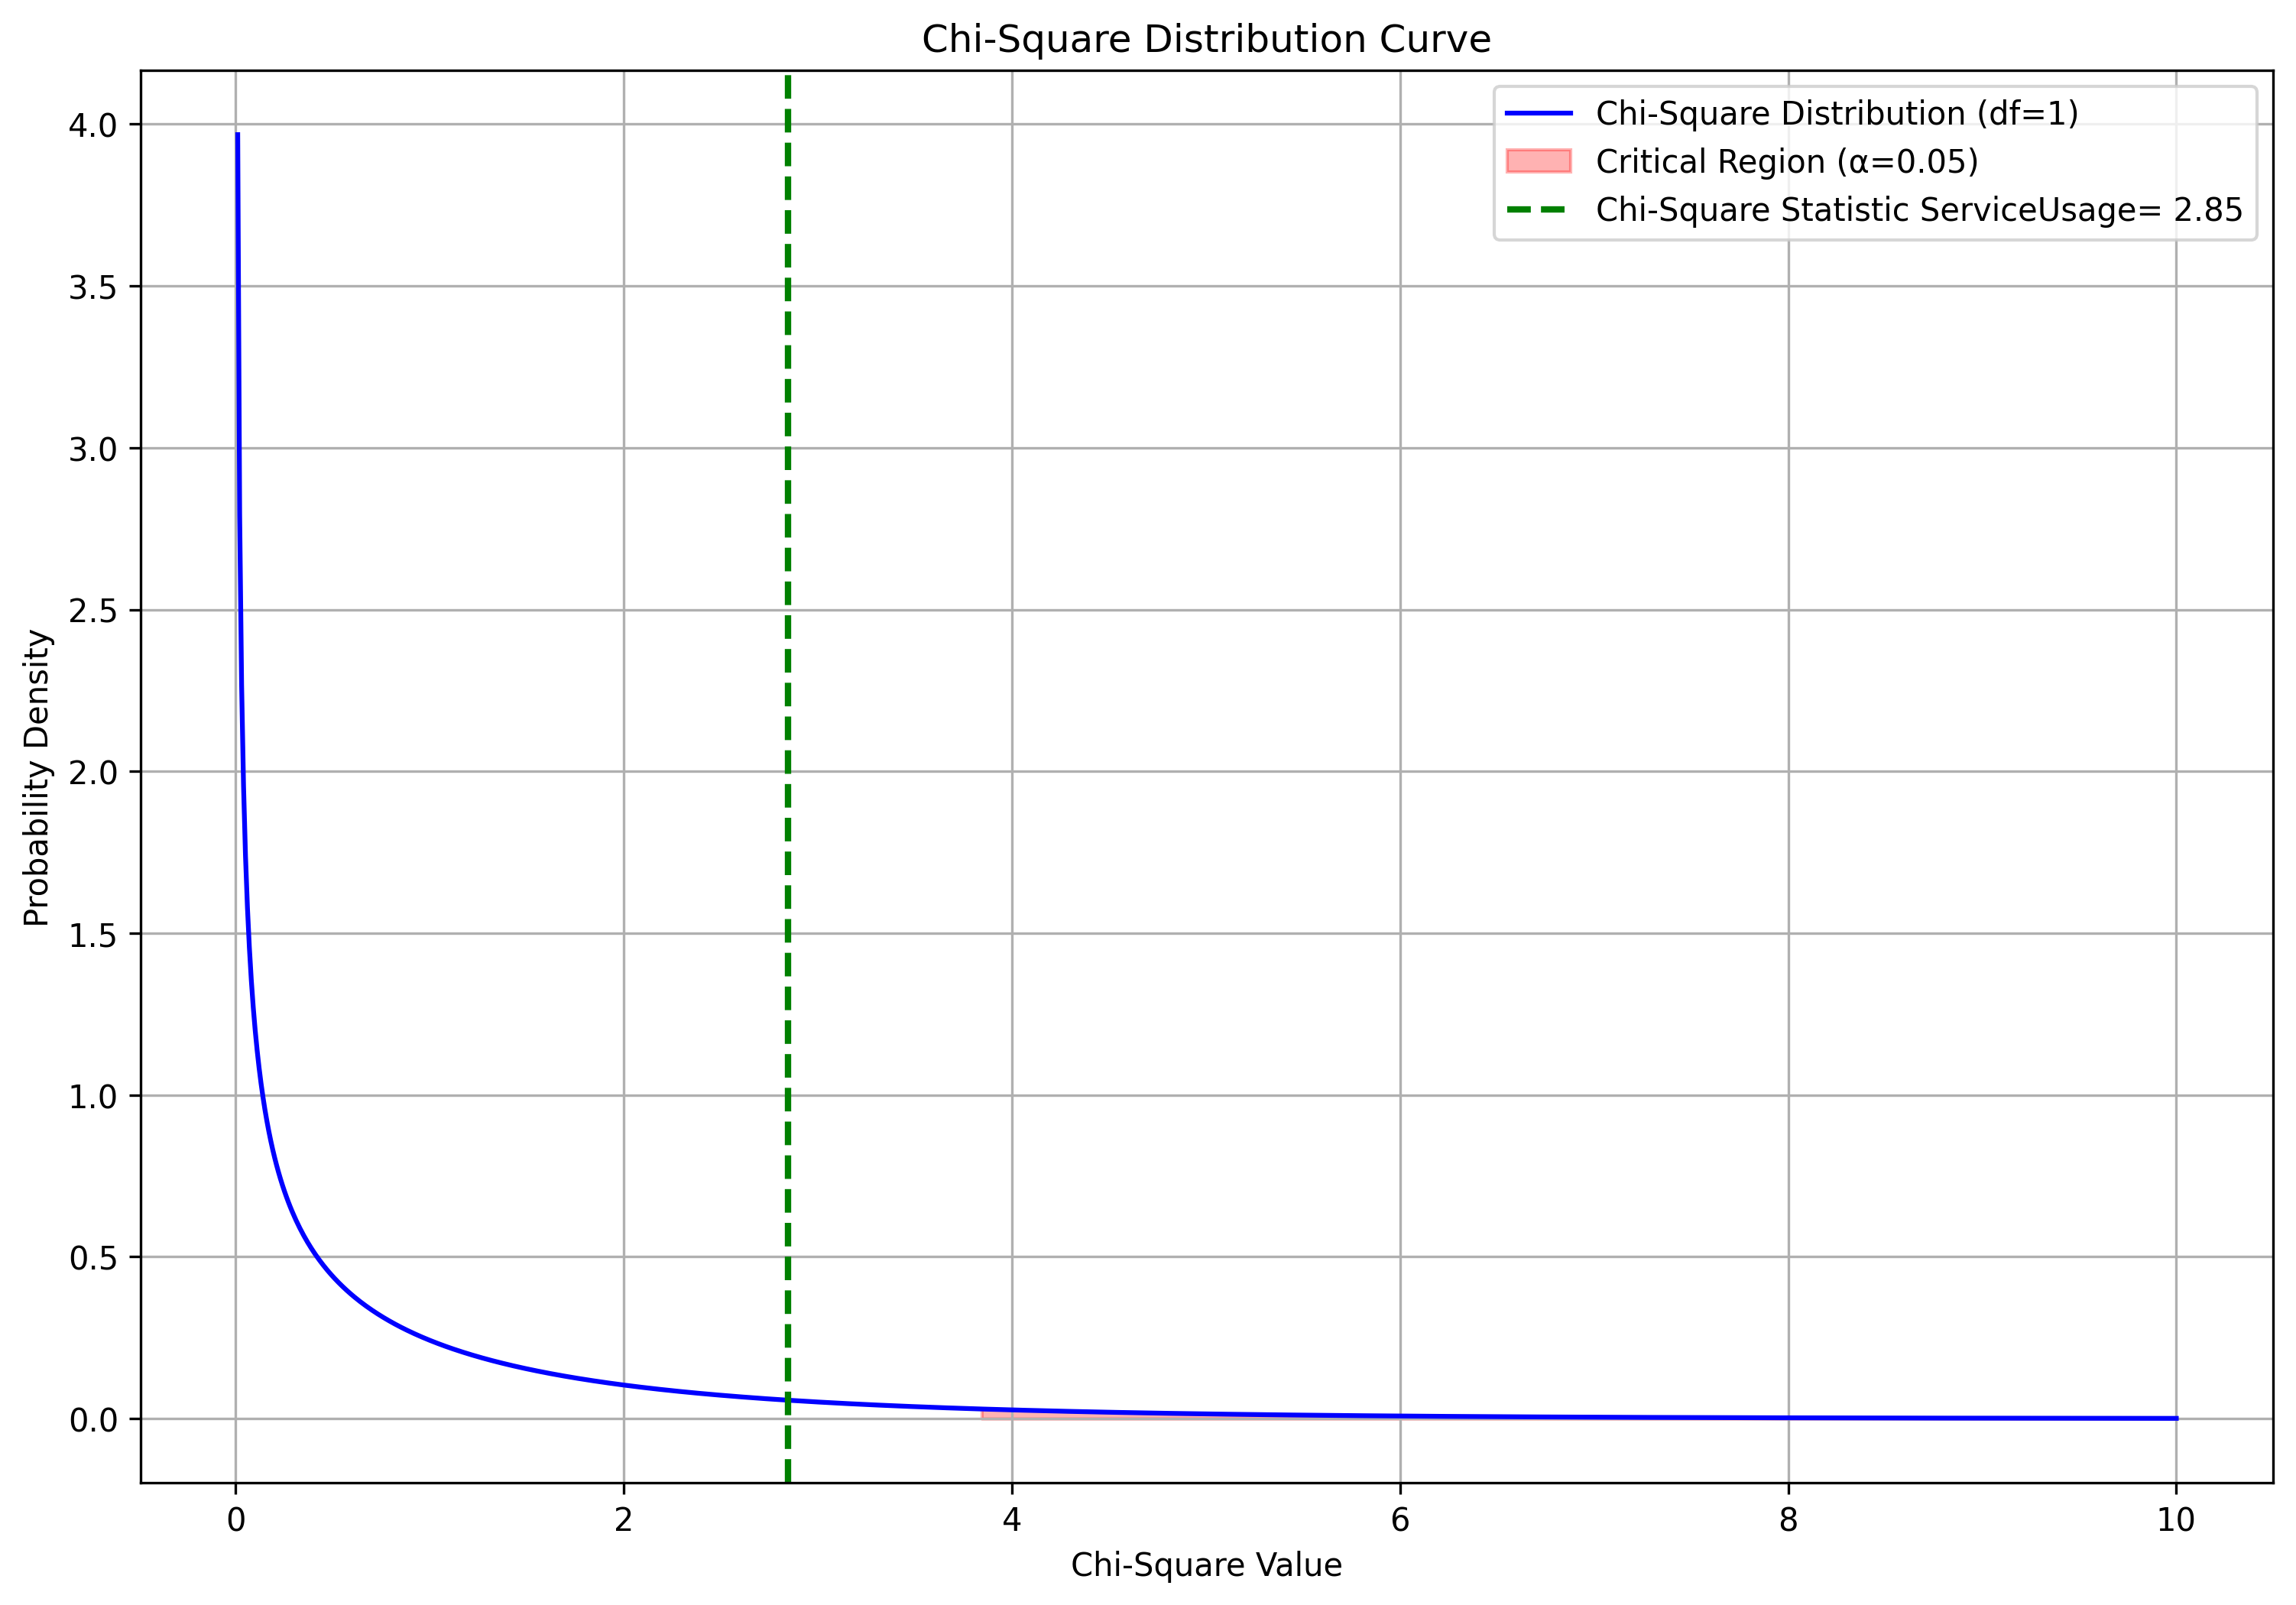
\includegraphics[width=0.49\textwidth]{Plots/Chi-Square_ServiceUsage.png}
    \caption{T-test distribution plot for LoginFrequency and DaysSinceLastLogin (left), and $\chi^2$ test result for ServiceUsage (right)}
    \label{fig:hypothesistesting}
\end{figure}

 As shown in Fig~\ref{fig:hypothesistesting}, As shown in Fig.~\ref{fig:hypothesistesting}, the t-test statistic for login frequency falls within the critical region($\alpha =0.05$), Therefore, the null hypothesis—that the mean values between churned and retained customers are the same—is rejected, indicating that login frequency may be a useful predictor of customer churn. However, DaysSinceLastLogin does not show a significant difference between churned and retained users, indicating that the time since the last login may not be a strong individual indicator of churn. Similarly, the $\chi^2$ test for ServiceUsage suggests that there is no strong relationship between service usage and churn status.

Moreover, LoginFrequency is normalised by dividing each value by the maximum LoginFrequency, providing a relative measure of customer engagement. Additionally, ServiceUsage is transformed using one-hot encoding to effectively represent categorical information.

\section{Classifier Training}

After preparing the enhanced features introduced above, we can analyse the correlation among the variables, and explore the impact of these features on churn prediction by comparing a baseline XGBoost model with an enhanced model trained on CTGAN-generated synthetic data. To address data imbalance, we generate additional churned user samples at 5x the original size using CTGAN, then merge them with the original dataset. Both models are trained using the same XGBoost hyperparameters.

\begin{table}[h]
    \centering
    \begin{tabular}{c|c|c}
        \hline
        & \textbf{Churned Customer} & \textbf{Retained Customer} \\
        \hline
        \textbf{Baseline Model Precision} & 0.27 & 0.80 \\
        \hline
        \textbf{Baseline Recall Rate} & 0.10 & 0.93 \\
        \hline
        \textbf{Feature Enhanced Model Precision} & 0.94 & 0.76 \\
        \hline
        \textbf{Feature Enhanced Model Recall} & 0.81 & 0.92 \\
        \hline
    \end{tabular}
    \caption{Comparison of precision and recall between the baseline and feature-enhanced models for churned and retained customers}
    \label{tab:metrics}
\end{table}

From Tab~\ref{tab:metrics} and AUC-ROC~\cite{BRADLEY19971145} Fig~\ref{fig:aucs}, the enhanced features significantly improve the accuracy of identifying churned customers by slightly sacrificing the accuracy in predicting retained customers,

\begin{figure}[h]
    \centering
    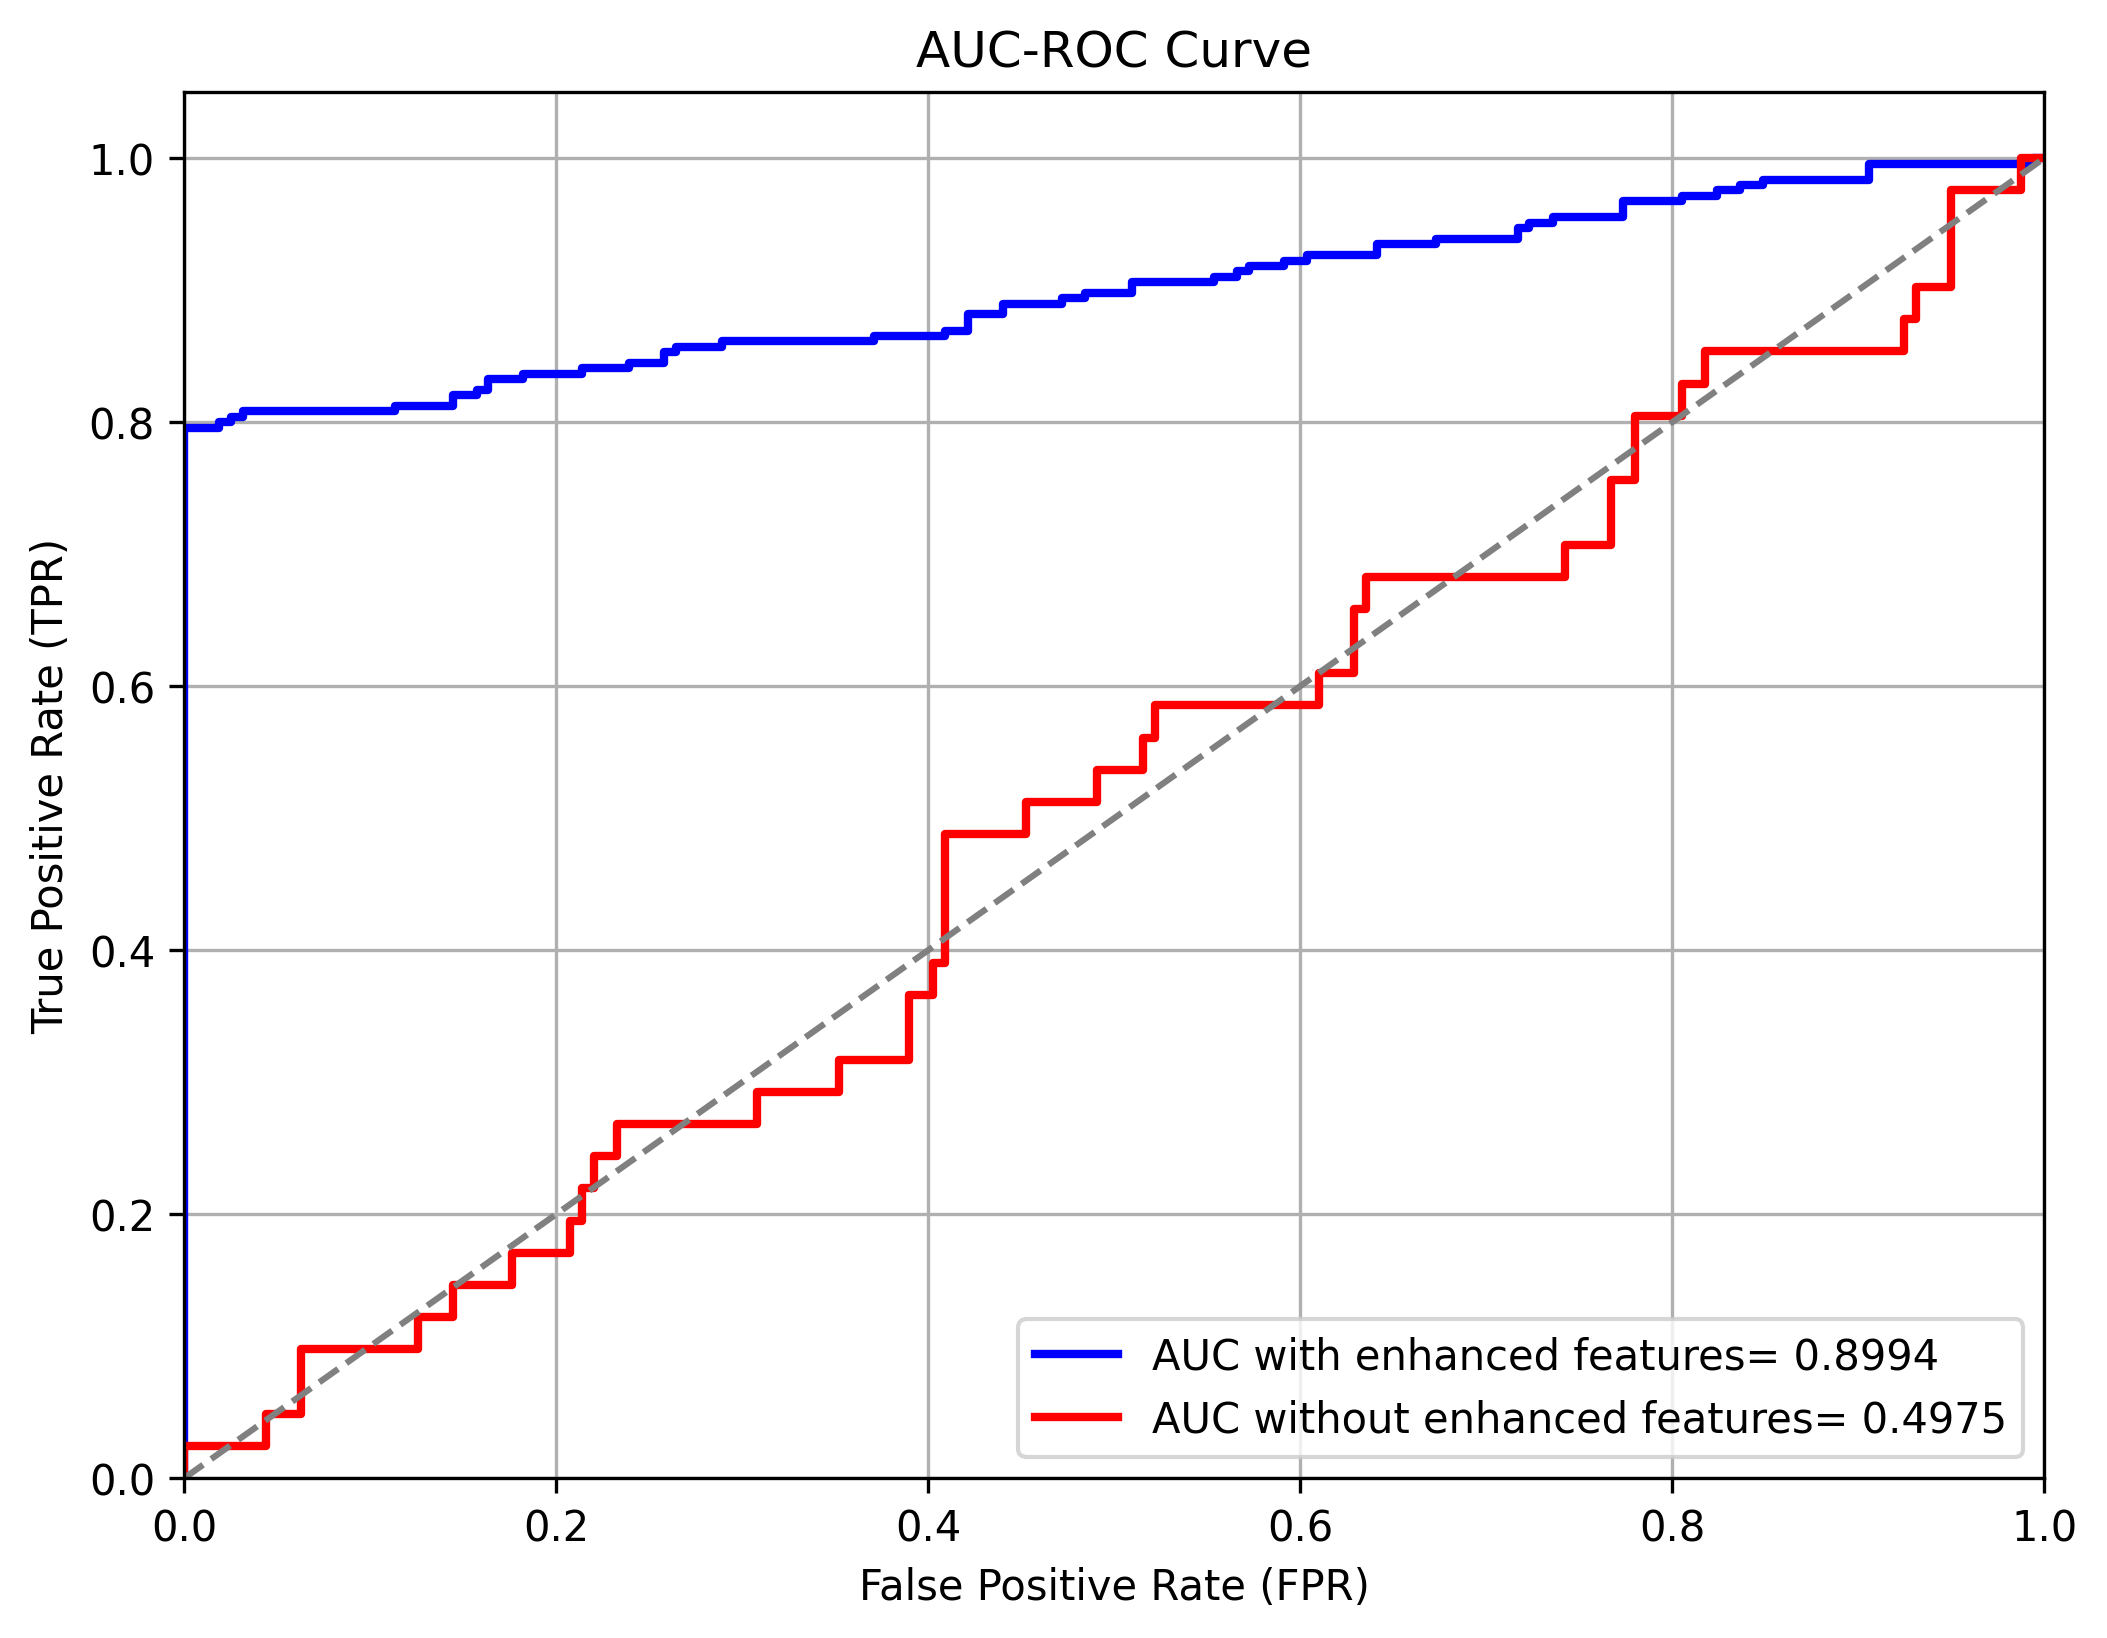
\includegraphics[width=0.49\textwidth]{Plots/AUCs.png}
    \caption{AUC-ROC plot for the baseline and feature-enhanced models}
    \label{fig:aucs}
\end{figure}

\begin{figure}[h]
    \centering
    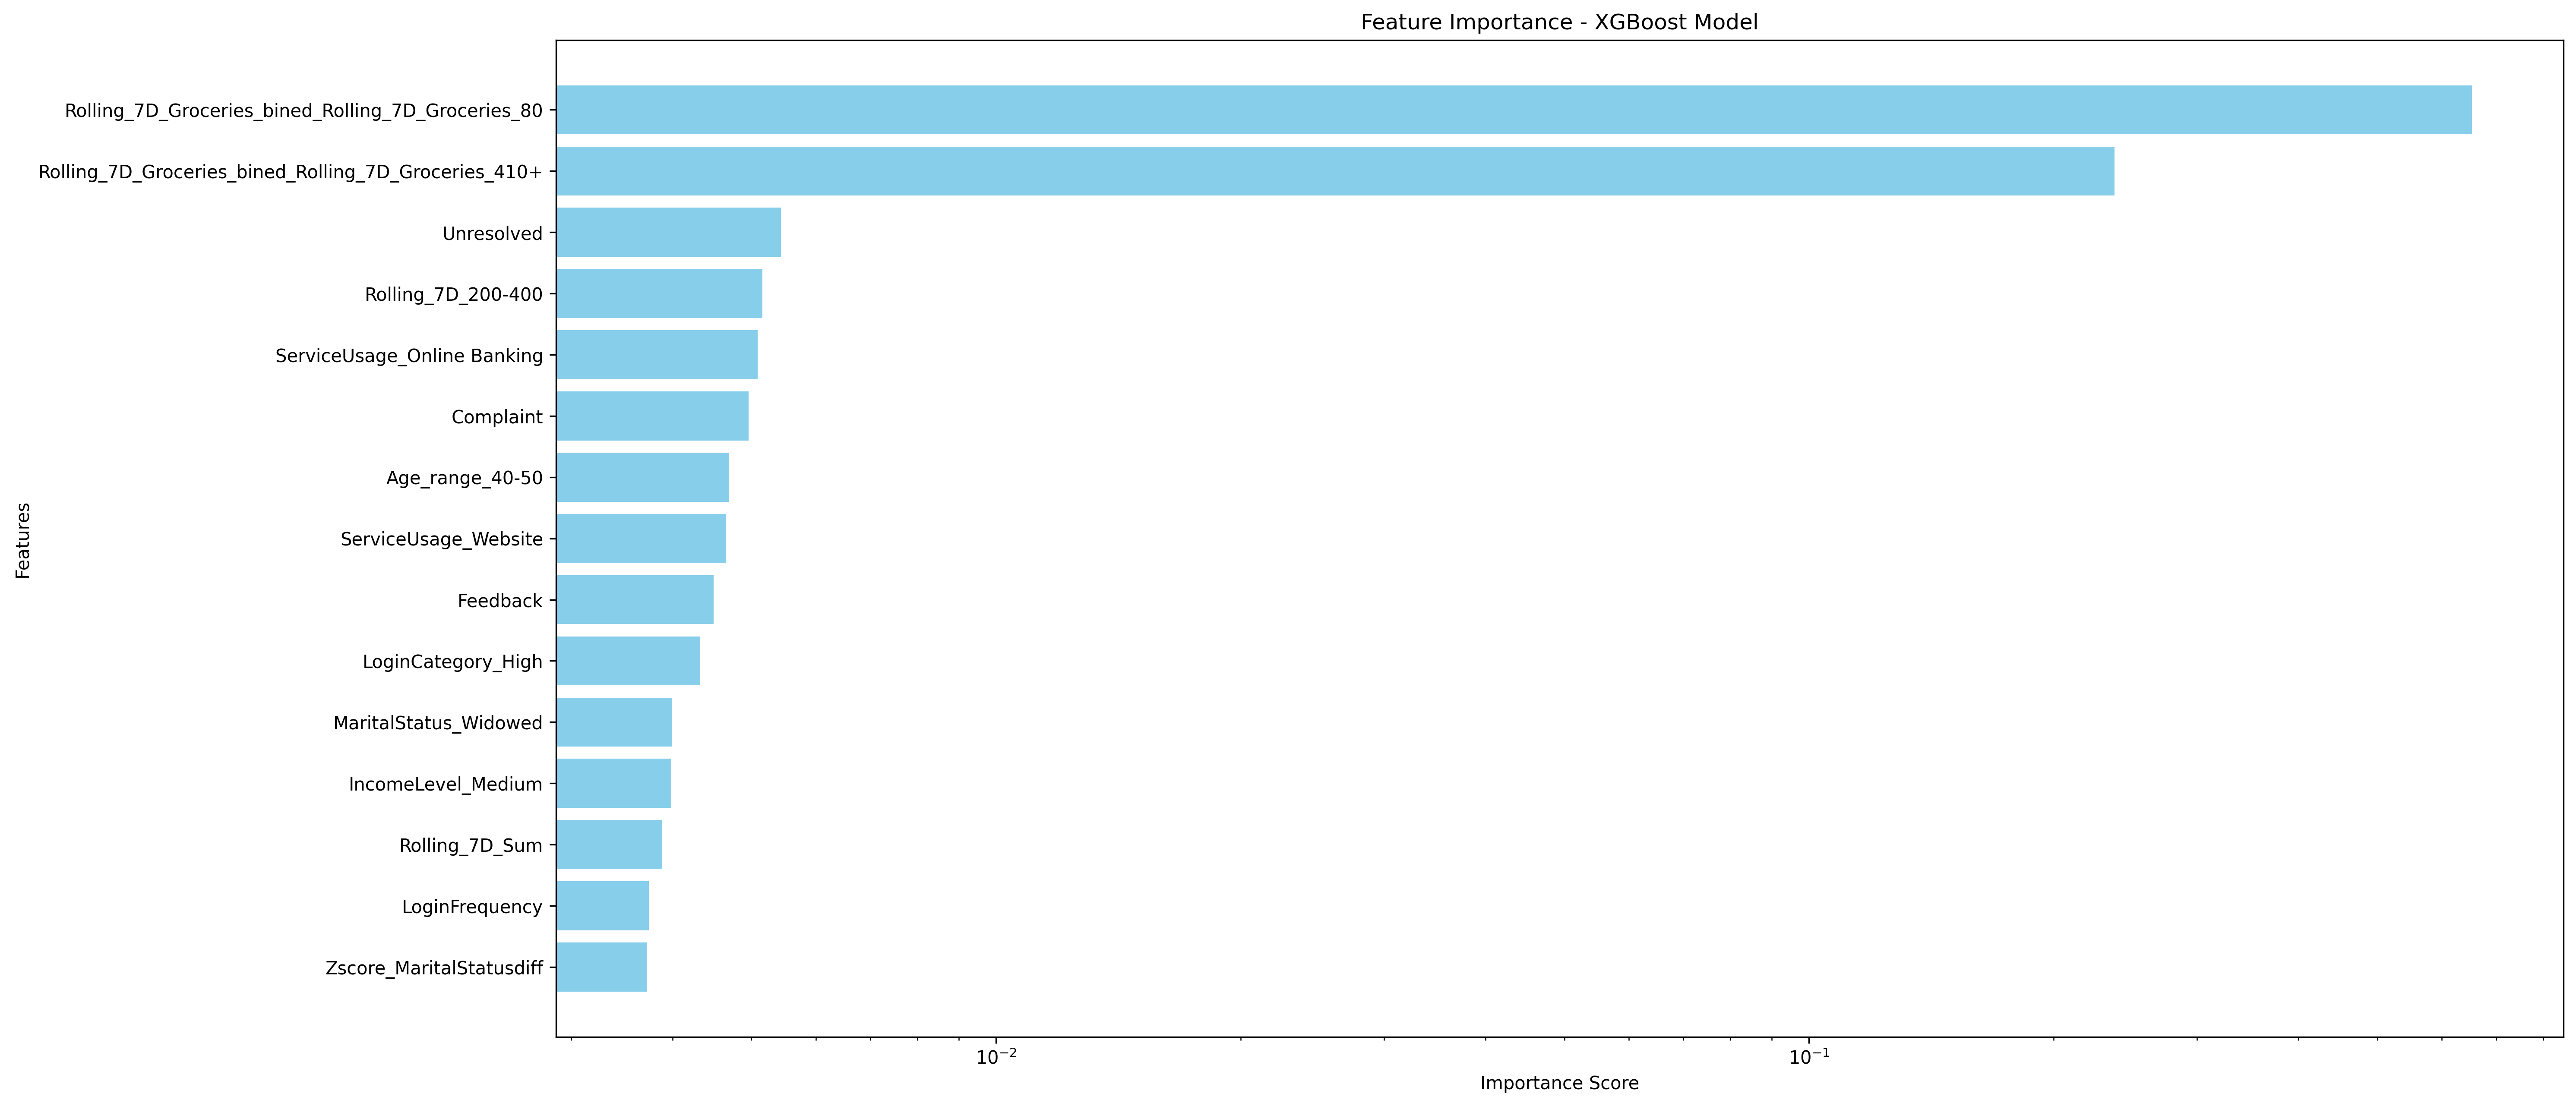
\includegraphics[width=0.96\textwidth]{Plots/importance_rank.png}
    \caption{importance rank of top 15 variables in the feature-enhanced model}
    \label{fig:rank}
\end{figure}

Fig~\ref{fig:rank} shows that recent grocery spending (Rolling\_7D\_Groceries) is the most influential factor in predictions, followed by customer service interactions (Unresolved issues, Complaints) and user engagement with online services (Online Banking, Website Usage). Demographic factors like age and marital status also play a role. 







\section{Conclusion}

This study shows the impact of statistical feature engineering in improving customer churn prediction. By applying techniques such as Z-score normalisation, Markov Chains, and so on, we extracted key predictive variables that enhanced model performance. The feature-enhanced XGBoost model, trained with CTGAN-generated synthetic data, showed significant improvements in identifying churned customers compared to the baseline model.

For business aspects, the findings indicate that factors like unresolved complaints, recent spending behaviour, and online engagement play crucial roles in churn prediction. These insights can help businesses develop targeted retention strategies, reducing customer attrition and improving long-term engagement.




% If using any of the following journal options:
%   wet, dap, dce, eds, prm, flw, jdm, psy, rsm
% then use the \printbibliography line instead of:

%\bibliography{example}

%\bibliography{example}
\printbibliography


\section{Appendix}

\subsection{Codes and additional plots}

\includepdf[pages=-]{Feature_Enhanced.pdf}
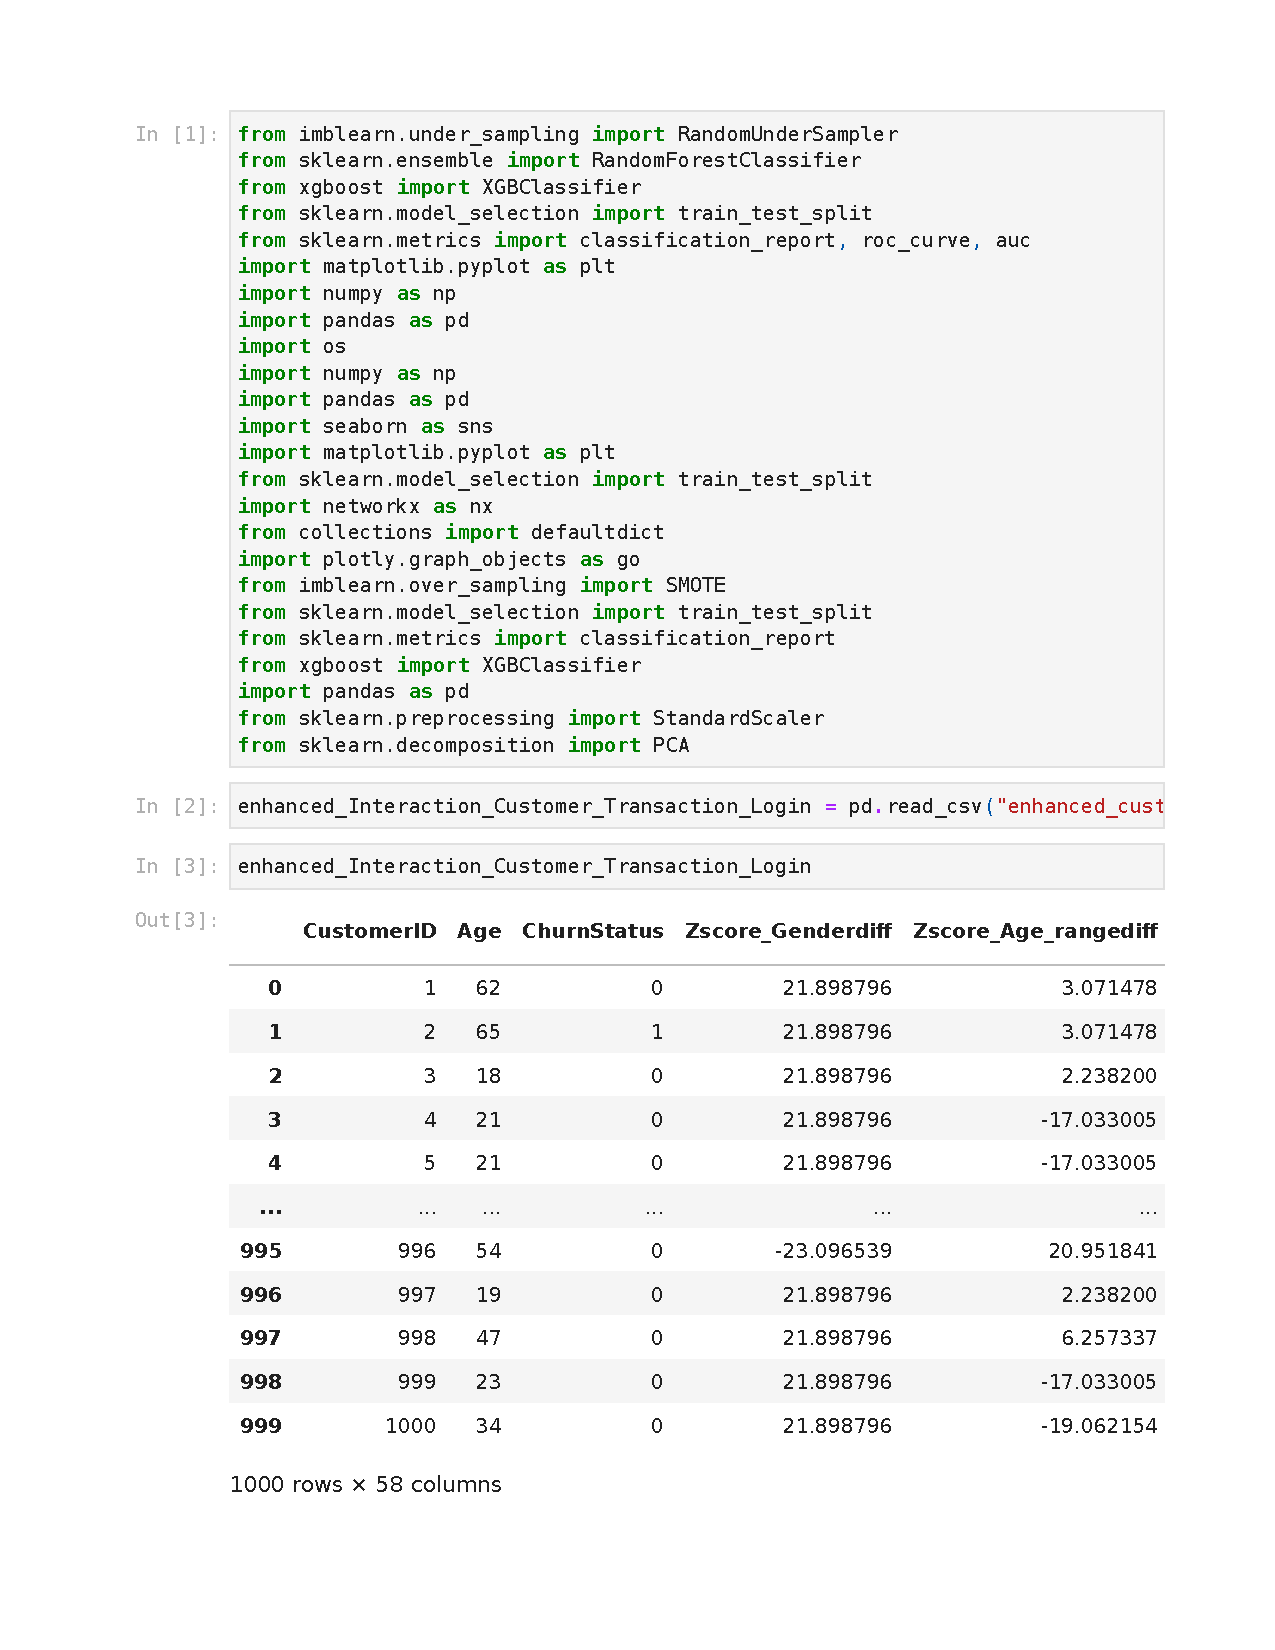
\includepdf[pages=-]{Training.pdf}


\subsection{Simulation Certificate}
Thanks to Vesna Perisic for the patient guidance during the term. Through this coursework, I successfully applied my knowledge to complete the Lloyds Bank job simulation combined with the coursework at the same time, which I believe will be very beneficial for my future career!

\begin{figure}[h]
    \centering
    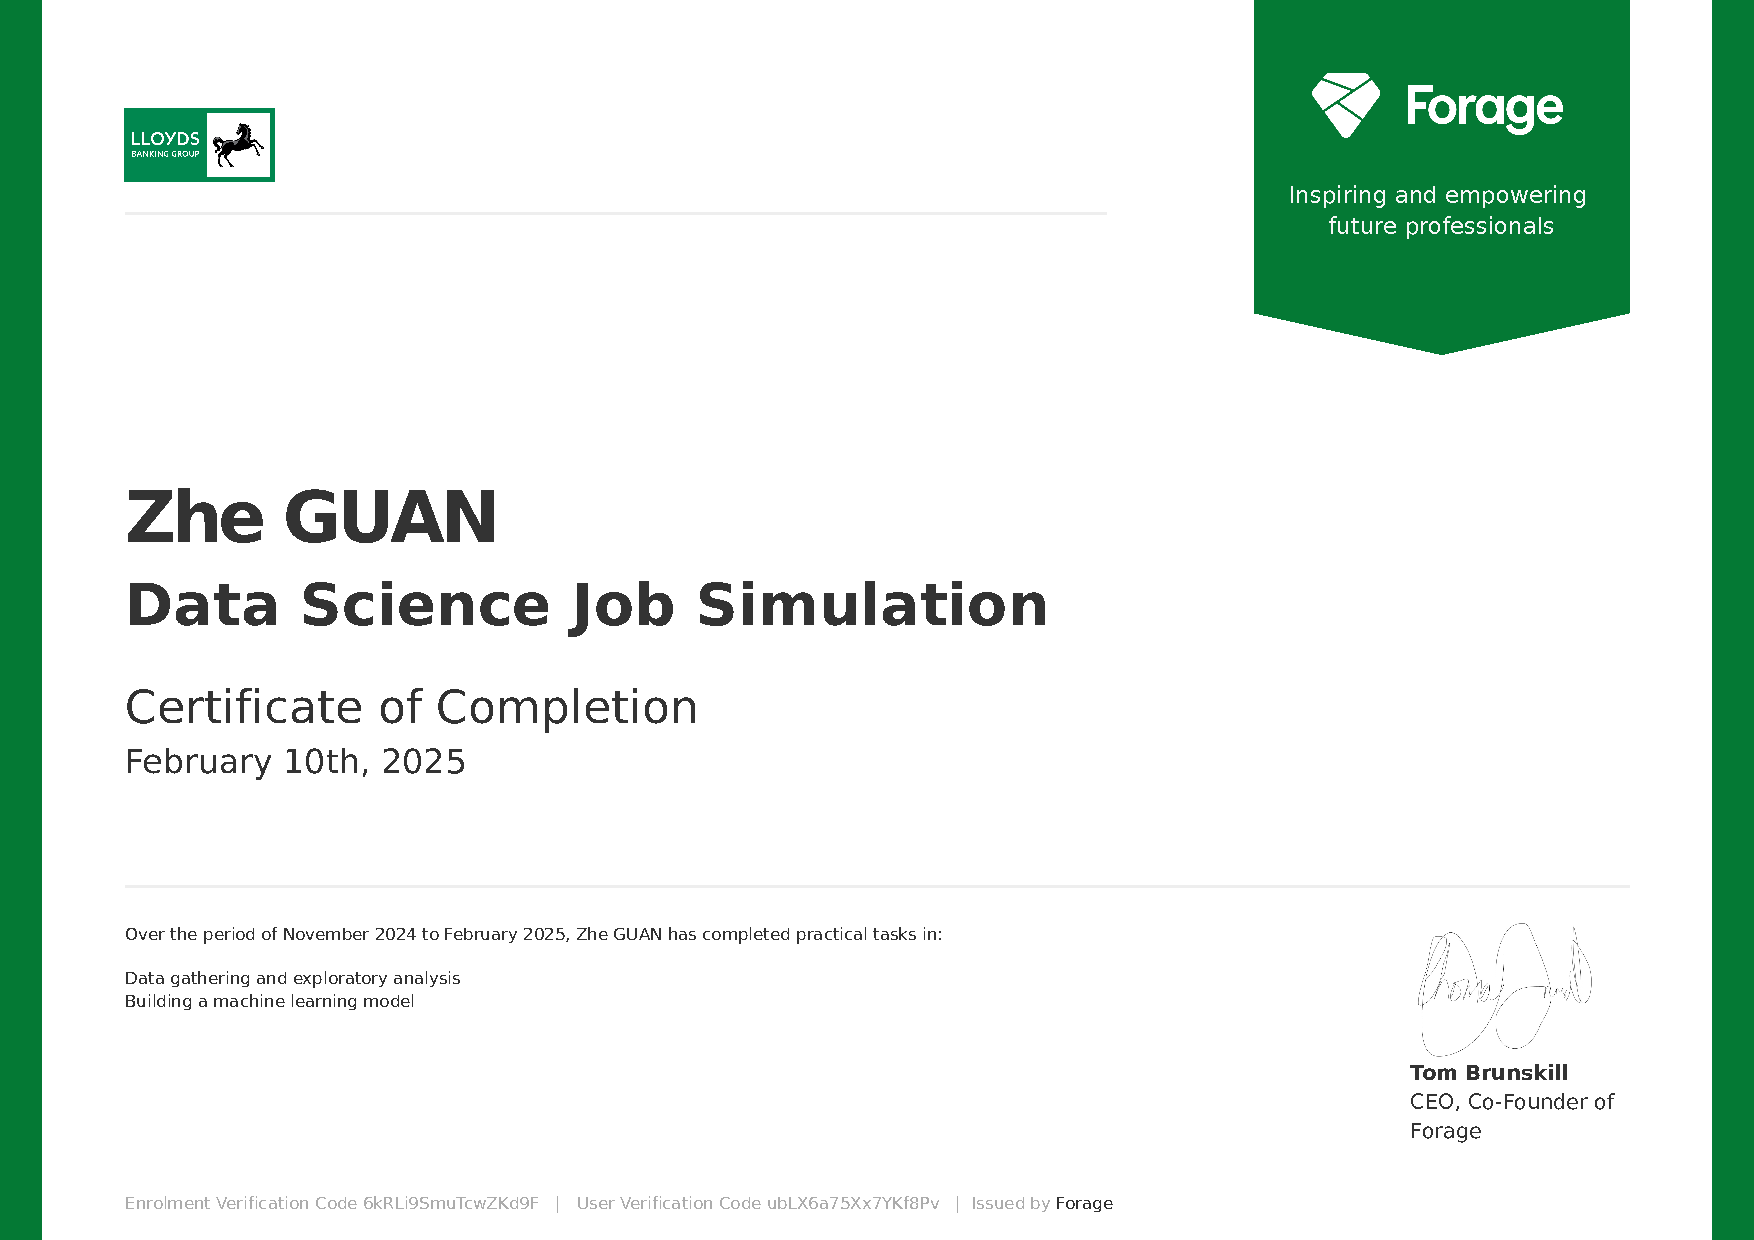
\includegraphics[width=0.96\textwidth]{LLoyd_Simulation_Certificate.pdf}
\end{figure}


\end{document}
